\documentclass[a4paper,11pt]{article}

%%%%%%%%%%%%%%%%%%%%%
% Encodage et langues
\usepackage[numbers]{natbib} % Charger avant babel
\usepackage[frenchb,english]{babel}
\usepackage[T1]{fontenc}
\usepackage[utf8]{inputenc}

%%%%%%%%%%%%%%%%%%%%%
% Liens et métadonnées
\usepackage[colorlinks=false, urlcolor=black, breaklinks, pagebackref, citebordercolor={0 0 0}, filebordercolor={0 0 0}, linkbordercolor={0 0 0}, pagebordercolor={0 0 0}, runbordercolor={0 0 0}, urlbordercolor={0 0 0}, pdfborder={0 0 0}]{hyperref}

%%%%%%%%%%%%%%%%%%%%%
% Mise en page et utilitaires
\usepackage{float}
\usepackage{amsmath}
\usepackage{amsfonts}
\usepackage{amssymb}
\usepackage{geometry}
\geometry{a4paper, margin=2.5cm, headheight=17pt}
\usepackage{graphicx}
\usepackage{icomma}
\usepackage{latexsym}
\usepackage{textcomp}
\usepackage{cancel}
\usepackage{color}
\usepackage{dsfont}
\usepackage{subfig}
\usepackage{caption}
\usepackage{booktabs}
\usepackage{longtable}
\usepackage{extarrows}
\usepackage{shorttoc}
\usepackage{listings}
\usepackage{xcolor}
\usepackage{enumitem}
\usepackage{lmodern}
\usepackage{moreverb}
\usepackage{fancyhdr}

% Rendre les listes moins "visuelles" et plus compactes (réduit la fatigue à la lecture)
\setlist[itemize]{label=\textendash, leftmargin=*, nosep}

\lstset{
	    basicstyle=\ttfamily\footnotesize,
	    breaklines=true,
	    frame=single,
    backgroundcolor=\color{gray!5},
    literate={é}{{\'e}}1 {è}{{\`e}}1 {à}{{\`a}}1 {ç}{{\c{c}}}1 {œ}{{\oe}}1 {ù}{{\`u}}1 {É}{{\'E}}1 {È}{{\`E}}1 {À}{{\`A}}1 {Ç}{{\c{C}}}1 {Œ}{{\OE}}1 {Ê}{{\^E}}1 {ê}{{\^e}}1 {î}{{\^i}}1 {ô}{{\^o}}1 {û}{{\^u}}1
}

\lstdefinelanguage{pseudo}{
    morekeywords={for,foreach,while,if,else,return},
    sensitive=false
}

\newcommand{\bigO}[1]{\ensuremath{\mathop{}\mathopen{}O\mathopen{}\left(#1\right)}}
\newcommand{\smallO}[1]{\ensuremath{\mathop{}\mathopen{}o\mathopen{}\left(#1\right)}}

\captionsetup{font=footnotesize}
\emergencystretch=1em

\setcounter{tocdepth}{3}

%%%%%%%%%%%%%%%%%%%%%
% Page de titre personnalisée
\makeatletter
\def\clap#1{\hbox to 0pt{\hss #1\hss}}%
\def\ligne#1{%
\hbox to \hsize{%
\vbox{\centering #1}}}%
\def\haut#1#2#3{%
\hbox to \hsize{%
\rlap{\vtop{\raggedright #1}}%
\hss
\clap{\vtop{\centering #2}}%
\hss
\llap{\vtop{\raggedleft #3}}}}%
\def\bas#1#2#3{%
\hbox to \hsize{%
\rlap{\vbox{\raggedright #1}}%
\hss
\clap{\vbox{\centering #2}}%
\hss
\llap{\vbox{\raggedleft #3}}}}%
\def\maketitle{%
\thispagestyle{empty}\vbox to \vsize{%
\haut{}{\@blurb}{}
\vfill
\vspace{0.5cm}
\hrule height 2pt
\vspace{0.2cm}
\par
\begin{center}
\fontseries{bx}
\huge \@title
\end{center}
\vspace{0.2cm}
\par
\hrule height 2pt
\par
\vspace{2cm}
\begin{center}
\Large
\textit{Auteurs:}
\end{center}
\begin{center}
\Large 
\@author
\par
\end{center}
\vspace{1cm}
\begin{center}
\Large
\textit{Encadrant:}
\end{center}
\begin{center}
\Large
Aurélien Delval
\par
\end{center}
\vspace{1cm}
\begin{center}
\Large
\textit{Responsables:}
\end{center}
\begin{center}
\Large 
Aurélien Delval / Hugo Bolloré / Pablo Oliveira
\par
\end{center}
\vfill
\vfill
\bas{}{\begin{flushright}
\large
\@date
\end{flushright}}{}
}%
\cleardoublepage
}
\def\date#1{\def\@date{#1}}
\def\author#1{\def\@author{#1}}
\def\title#1{\def\@title{#1}}
\def\location#1{\def\@location{#1}}
\def\blurb#1{\def\@blurb{#1}}
\date{\today}
\author{Jianye Shi, Hao Qian, Xiang Bian, Abdennour Boulmis}
\title{Rapport de Projet : MLP et moteur d'autodiff appliqués à MNIST}
\location{}\blurb{%
\begin{center}

\includegraphics[width=20em]{Images/Logo_UVSQ.jpg}\\[0.5cm]
\end{center}
}%
\makeatother

%%%%%%%%%%%%%%%%%%%%%
% En-têtes et pieds de page
\pagestyle{fancy}
\fancyhf{}
\fancyhead[L]{M1 CHPS -- UVSQ 25/26}
\fancyhead[R]{\leftmark}
\fancyfoot[C]{\thepage}
\renewcommand{\headrulewidth}{0.4pt}
\renewcommand{\footrulewidth}{0pt}
\setlength{\headheight}{17pt}

\begin{document}

\maketitle

\renewcommand{\contentsname}{Sommaire}
\tableofcontents
\newpage
\listoffigures
\listoftables
\newpage

\section{Introduction}
Ce rapport présente l'implémentation \textit{from scratch} d'un Perceptron Multicouche (MLP) et d'un moteur de différenciation automatique appliqué au jeu de données MNIST \cite{lecun1998}. Réalisé dans le cadre du Master 1 CHPS à l'Université Paris-Saclay, ce projet vise un double objectif : comprendre les mécanismes internes de l'apprentissage profond (propagation, rétropropagation) et s'initier à l'optimisation de code bas niveau, sans dépendre de bibliothèques tierces.

\section*{Plan du document}
Le rapport s'articule autour de quatre axes :
\begin{enumerate}[label=\textbf{\arabic*.}, leftmargin=*, nosep]
  \item \textbf{État de l'art} : présentation du problème MNIST et des fondements théoriques du MLP.
  \item \textbf{Implémentation} : architecture du moteur d'autodifférentiation et conception logicielle.
  \item \textbf{Expérimentations} : validation de la convergence (Machine Learning) et analyse des performances (HPC).
  \item \textbf{Organisation} : répartition des tâches et déroulement du projet.
\end{enumerate}
Une conclusion, des annexes techniques et un glossaire complètent ce document.

\vspace{3cm}

\section{Contexte et État de l'art}

\subsection{Introduction au problème}
Au cours des dernières décennies, l'apprentissage automatique a connu un développement considérable, principalement grâce aux progrès réalisés dans le domaine des réseaux de neurones artificiels. Parmi les problèmes emblématiques de ce domaine figure la reconnaissance de chiffres manuscrits, couramment étudiée à l'aide du jeu de données MNIST \cite{lecun1998}, devenu un standard pour les tâches de classification. Ce travail vise à présenter les approches classiques permettant de résoudre ce problème, en commençant par le perceptron multicouche (MLP), avant d'aborder ses principales variantes et l'évolution des modèles plus récents.

\subsection{Concept de la méthode classique}
Le problème MNIST consiste à classer des images de chiffres manuscrits ($28 \times 28$ pixels) dans dix catégories correspondant aux chiffres 0 à 9. Pour résoudre ce problème, on utilise un perceptron multicouche (MLP), c'est-à-dire un réseau de neurones constitué de plusieurs neurones artificiels organisés en couches (entrée, cachées, sortie).

Chaque neurone calcule une combinaison linéaire de ses entrées, à laquelle il applique ensuite une fonction d'activation non linéaire.
Soit $x$ le vecteur d'entrée, $w$ le vecteur de poids et $b$ le biais. La sortie $y$ d'un neurone est donnée par :
\[ y = \sigma(w \cdot x + b) \]

\paragraph{Passage au calcul matriciel}
On commence par le cas d'un seul exemple. Une image MNIST de taille $28\times 28$ est vectorisée (\textit{flattened}) en un vecteur d'entrée $x\in\mathbb{R}^{1\times 784}$. Pour une couche entièrement connectée comportant $n$ neurones, on introduit une matrice de poids $W\in\mathbb{R}^{784\times n}$ et un biais $b\in\mathbb{R}^{1\times n}$. La pré-activation s'écrit alors :
\[ z = xW + b \]
où $z\in\mathbb{R}^{1\times n}$. Cette transformation correspond à une application affine de l'espace des pixels (dimension 784) vers un espace de représentation de dimension $n$, avant l'application de la non-linéarité $\sigma$.

Dans la pratique, un traitement séquentiel (image par image) exploite imparfaitement les ressources matérielles. Afin d'augmenter le débit (\textit{throughput}), on recourt au calcul par \textit{mini-batchs} (\textit{mini-batches}), qui permet de reformuler une suite de produits vecteur-matrice en un unique produit matrice-matrice, particulièrement optimisé (SIMD, multi-cœurs, BLAS, et, le cas échéant, GPU).

Plus précisément, en regroupant $N$ exemples, on définit la matrice d'entrées $X\in\mathbb{R}^{N\times 784}$. La propagation avant se généralise en :
\[ Y = \sigma(XW + \mathbf{1}_N b) \]
où $\mathbf{1}_N\in\mathbb{R}^{N\times 1}$ désigne un vecteur de 1 et $\mathbf{1}_N b$ formalise la diffusion (\textit{broadcast}) du biais sur l'ensemble des $N$ exemples.

Pour clarifier ce mécanisme, la figure suivante illustre d'abord le cas $xW$, puis son extension naturelle au cas matriciel avec $XW$.

\begin{figure}[H]
  \centering
  
\includegraphics[width=0.7\textwidth]{Images/LayersOfMLP.png}
  \caption{Architecture d'un Perceptron Multicouche (MLP) avec couches cachées \cite{cour-GLHPC}.}
  \label{fig:layers_of_mlp}
\end{figure}

Cette figure illustre la structure hiérarchique du modèle (schéma purement illustratif : pour MNIST, chaque entrée est un vecteur de dimension 784, et un mini-batch correspond à une matrice $X$ de dimensions $N \times 784$) :

\textbf{Couche d'entrée} ($x_0$ à $x_3$) : reçoit les données brutes (ici les pixels d'une image).

\textbf{Couches cachées} : couches intermédiaires où le réseau apprend des représentations abstraites ; chaque neurone est connecté à tous les neurones de la couche précédente (\textit{fully connected}).

\textbf{Couche de sortie} ($y$) : produit la prédiction finale (probabilités des classes pour MNIST).

Bien que le schéma montre des connexions individuelles, notre implémentation vectorise ces opérations sous forme de produits matriciels $X \cdot W$. C'est cette opération matricielle que nous optimisons intensivement dans ce projet (BLAS, OpenMP).

L'objectif de l'apprentissage est de minimiser une fonction de \textit{loss} (\textit{loss}) $L$, qui quantifie l'écart entre les prédictions du modèle et les étiquettes réelles. Minimiser $L$ revient donc à réduire cet écart sur les données d'entraînement (et, idéalement, à améliorer la capacité de généralisation sur des exemples non vus). Dans la suite, la rétropropagation (\textit{backpropagation}) \cite{rumelhart1986} permet de calculer le gradient $\nabla L$ par rapport à tous les paramètres afin d'effectuer cette minimisation.

\paragraph{Règle de la chaîne (\textit{chain rule})}
Le réseau peut se voir comme une composition de fonctions $f(x) = f_n(f_{n-1}(\dots f_1(x)))$. Le gradient se calcule en remontant de la fin vers le début via la règle de la chaîne :
\[ \frac{\partial L}{\partial x} = \frac{\partial L}{\partial y} \cdot \frac{\partial y}{\partial x} \]
Cela conduit naturellement à une représentation sous forme de \textbf{graphe de calcul} (DAG), où chaque nœud est une opération élémentaire, connaissant ses parents et sa dérivée locale. Lors de la phase \textit{backward}, nous propageons le gradient accumulé depuis la perte jusqu'aux feuilles (les poids). Dans le cas général, exprimer analytiquement le gradient d'un réseau profond est difficile et source d'erreurs. L'autodiff permet de le calculer automatiquement en appliquant systématiquement la règle de la chaîne, sans dériver explicitement les formules pour chaque architecture (p. ex. PyTorch, TensorFlow).

\paragraph{Exemple : graphe de calcul et autodiff}
Un exemple détaillé est donné en Annexe~\ref{app:autodiff_example}.

\subsection{Présentation des éléments modulables du MLP}

Après avoir décrit le fonctionnement général du MLP et les principes du calcul de gradient, nous présentons maintenant les différents éléments modulables de cette architecture.

\subsubsection{Fonctions d'activation}
Les fonctions d'activation introduisent la non-linéarité dans le réseau. Elles sont cruciales pour deux raisons :
\begin{enumerate}
    \item \textbf{Non-linéarité} : Sans elles, une superposition de couches linéaires resterait une simple transformation linéaire unique ($W_2(W_1 x) = W'x$), incapable de modéliser des problèmes complexes (comme XOR ou MNIST).
    \item \textbf{Recadrage des valeurs} : Elles permettent souvent de maintenir les activations dans une plage bornée (p. ex. $[0,1]$ pour la sigmoïde), évitant l'explosion des valeurs lors de la propagation dans des réseaux profonds.
\end{enumerate}

\textbf{Sigmoïde} : transforme l'entrée en une valeur entre 0 et 1, mais peut provoquer la saturation des gradients. 

\textbf{Tanh} : centrée sur zéro, elle améliore souvent la convergence mais reste sujette au même problème de saturation. 

\textbf{ReLU} (\textit{Rectified Linear Unit}) : ne conserve que les valeurs positives ($ReLU(x) = \max(0, x)$) ; elle accélère l'apprentissage et constitue aujourd'hui un choix standard \cite{goodfellow2016}.

\subsubsection{Algorithmes de descente de gradient}\label{sec:theory_sgd}
L'apprentissage consiste à minimiser la \textit{loss} grâce à la descente de gradient. L'algorithme met à jour les paramètres $\theta$ (poids et biais) itérativement :
\[ \theta_{t+1} = \theta_t - \eta \cdot \nabla_\theta L \]
où $\eta$ est le \textbf{taux d'apprentissage} (\textit{learning rate}).
\begin{itemize}
    \item Un $\eta$ trop grand accélère la convergence mais risque de provoquer des oscillations, voire une divergence.
    \item Un $\eta$ trop petit garantit la stabilité mais ralentit considérablement l'apprentissage.
\end{itemize}

\begin{lstlisting}[language=pseudo, caption={Algorithme simplifié (SGD)}]
Pour chaque epoch:
  Pour chaque mini-batch (X, Y):
    1. Forward: P = Model(X)
    2. Loss: L = LossFn(P, Y)
    3. Backward: Calculer les gradients via autodiff
    4. Update: W = W - learning_rate * dL/dW
\end{lstlisting}

Si ce projet se concentre sur la méthode \textbf{SGD}, il convient de citer les évolutions majeures de l'état de l'art :
\begin{itemize}
    \item \textbf{SGD} (\textit{Stochastic Gradient Descent}) : met à jour les poids après chaque \textit{mini-batch} (\textbf{méthode implémentée}).
    \item \textbf{Momentum} : ajoute une inertie pour lisser les oscillations et accélérer la convergence.
    \item \textbf{Adam} : combine Momentum et adaptation du taux d'apprentissage ; optimisateurs standards actuels.
\end{itemize}

\subsection{Positionnement et Périmètre}
Bien que les réseaux convolutionnels (CNN), introduits par LeCun \textit{et al.} (LeNet-5 \cite{lecun1998}), dominent la reconnaissance d'images grâce à leur invariance spatiale ($>99\%$ de réussite), le Perceptron Multicouche (MLP) reste le modèle pédagogique de référence. Il permet de maîtriser les concepts fondamentaux : calcul matriciel, non-linéarité et rétropropagation du gradient.

Notre projet se concentre ainsi sur l'implémentation \textit{from scratch} d'un pipeline complet :
\begin{enumerate}[label=\itshape\alph*), nosep]
  \item moteur de tenseurs et d'autodifférentiation,
  \item architecture modulaire (couches, activations, optimiseur, loss),
  \item boucle d'entraînement optimisée (SGD, CrossEntropy, DataLoader, MiniBatch).
\end{enumerate}

\clearpage

\section{Implémentation}

\subsection{Architecture Globale}
Le projet implémente un moteur de \textit{Deep Learning} complet en C++ moderne, privilégiant la compréhension des mécanismes bas niveau et la performance. Le choix du C++ est motivé par son contrôle fin de la mémoire et sa capacité à produire un code efficace, en cohérence avec l'orientation \emph{calcul haute performance} de l'UE. L'architecture (Fig.~\ref{fig:uml}) s'articule autour de trois couches : le noyau de calcul (\texttt{Matrix}), le graphe d'autodiff (\texttt{Node}/\texttt{MathOps}) et les abstractions de plus haut niveau (couches, \textit{loss}, optimiseur, boucle d'entraînement).

\begin{figure}[H]
  \centering
  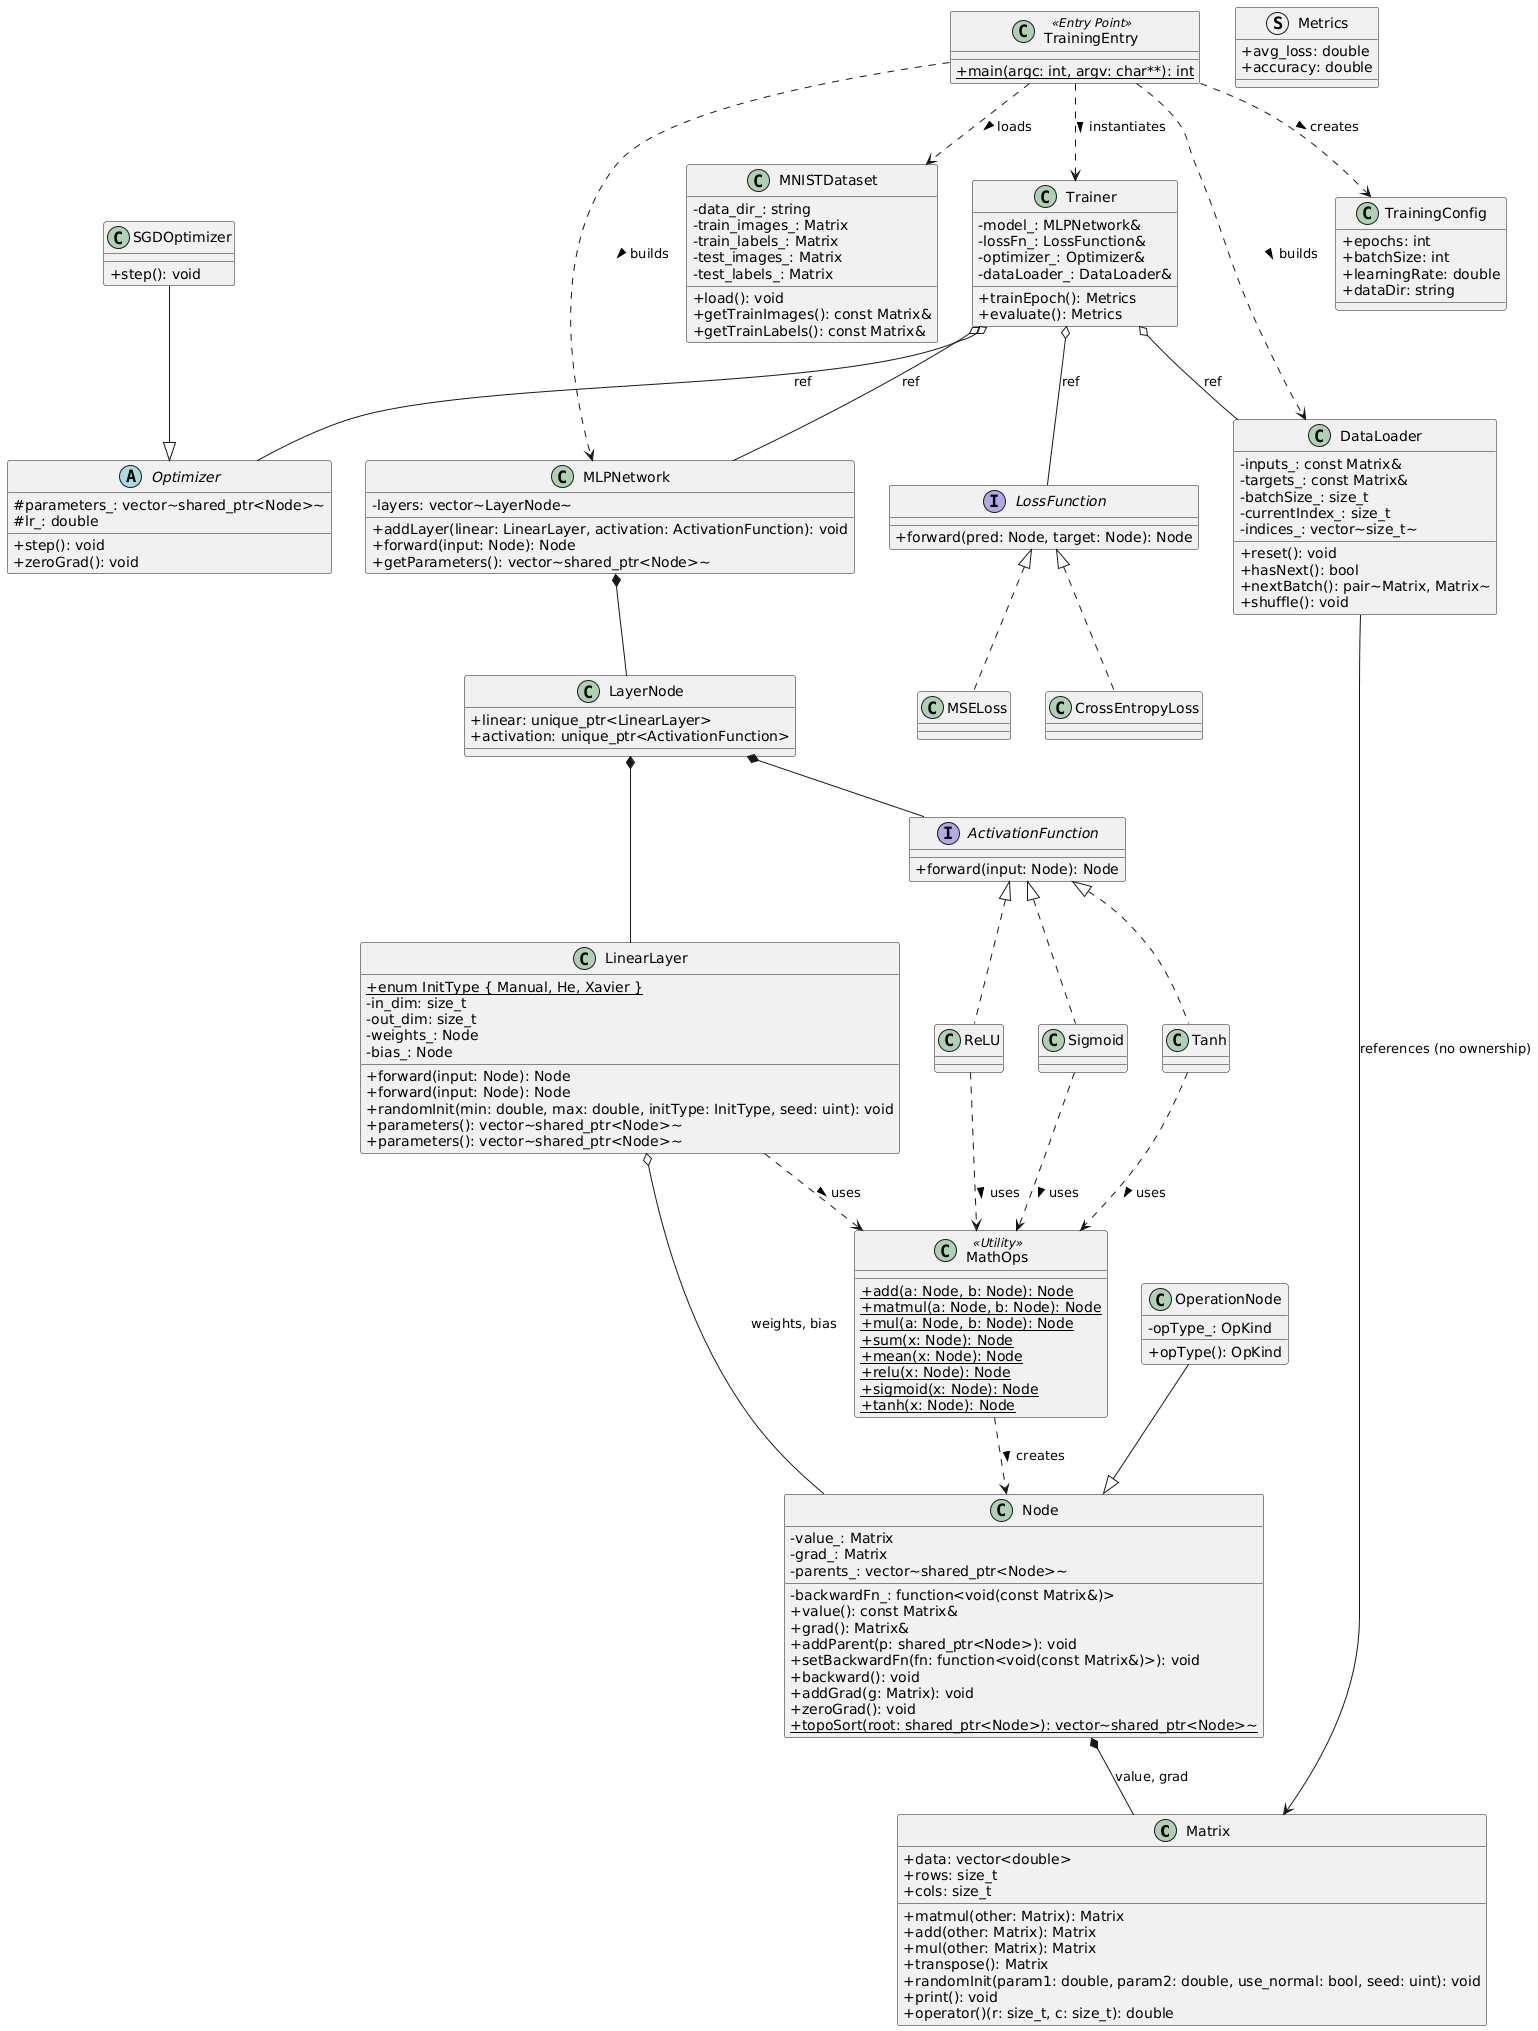
\includegraphics[width=0.9\textwidth]{Images/conception_detaillee.png}
  \caption{Architecture logicielle : du calcul matriciel (bas niveau) au pipeline d'entraînement.}
  \label{fig:uml}
\end{figure}

\subsection{Noyau de Calcul : Matrix}
La classe \texttt{Matrix} constitue la brique fondamentale. Pour optimiser l'utilisation des caches CPU (localité spatiale) et permettre la vectorisation (SIMD), les données sont stockées dans un conteneur contigu (\texttt{std::vector<double>}).
Afin d'analyser l'impact des optimisations, nous avons implémenté plusieurs versions de la multiplication matricielle (\texttt{matmul}), sélectionnables à l'exécution : une version naïve (triple boucle) à but pédagogique, et des versions performantes exploitant OpenMP et les bibliothèques BLAS. L'initialisation des poids suit des stratégies robustes (He pour ReLU, Xavier pour Sigmoid/Tanh) et intègre une gestion déterministe de l'aléatoire (\textit{seed}) pour assurer la reproductibilité.
\par\smallskip
\noindent Concrètement, la méthode \texttt{randomInit} applique une mise à l'échelle dépendante du fan-in : pour He, $\mathrm{Var}(W)=2/n_{in}$ (adaptée à ReLU) ; pour Xavier, $\mathrm{Var}(W)=1/n_{in}$ (adaptée à Sigmoid/Tanh). La graine est explicitement contrôlée afin de reproduire à l'identique les poids initiaux entre deux exécutions.

\subsection{Autodifférentiation : Node et MathOps}
Le moteur d'\textit{autodiff} repose sur un Graphe Acyclique Dirigé (DAG) dynamique. Chaque \texttt{Node}, géré via des pointeurs intelligents (\texttt{std::shared\_ptr}), stocke sa valeur, son gradient et ses dépendances.
L'originalité de l'implémentation réside dans l'utilisation d'expressions Lambda pour définir la rétropropagation (\textit{backpropagation}). Lors du passage avant (\textit{forward}), le contexte local est capturé efficacement par la fermeture (\textit{closure}), évitant la création de classes dédiées pour chaque opération.

\begin{lstlisting}[language=C++, caption={Rétropropagation via Lambda (MathOps)}]
// Exemple pour Mul (y = a * b) : capture du contexte {a, b}
node->setBackwardFn([a, b](const Matrix& grad){
    // Règle de la chaîne : dL/da = grad * b, dL/db = grad * a
    a->addGrad(grad.mul(b->value()));
    b->addGrad(grad.mul(a->value()));
});
\end{lstlisting}

La rétropropagation est déclenchée par un tri topologique du graphe (méthode \texttt{topoSort}), garantissant un parcours correct des dépendances sans récursion profonde. Pour faciliter l'analyse du graphe, les nœuds d'opérations sont identifiés par un type (\texttt{OperationNode} / \texttt{OpKind}). Enfin, certaines opérations (p. ex. \texttt{add}) gèrent une diffusion (\textit{broadcasting}) simple afin de supporter l'ajout du biais sur un mini-batch.

\subsection{Modélisation et Entraînement}
Le réseau est construit par composition de modules. \textbf{Couches :} \texttt{LinearLayer} encapsule les paramètres (poids, biais), et l'interface \texttt{ActivationFunction} permet d'interchanger les non-linéarités (ReLU, Sigmoid, Tanh) via le polymorphisme. La combinaison « couche linéaire + activation » est encapsulée dans \texttt{LayerNode}, et le modèle complet est représenté par \texttt{MLPNetwork} (séquence de \texttt{LayerNode}).
\par\smallskip
\noindent\textbf{Entraînement :} \texttt{Trainer} orchestre la boucle d'apprentissage. Les données sont chargées par \texttt{MNISTDataset} et regroupées en mini-batchs via \texttt{DataLoader}. La \textit{loss} est définie par l'interface \texttt{LossFunction} (implémentations \texttt{MSELoss} et \texttt{CrossEntropyLoss}), tandis que la mise à jour des paramètres est assurée par \texttt{Optimizer} (implémentation \texttt{SGDOptimizer}). À chaque mini-batch, le pipeline exécute : \textit{forward} $\rightarrow$ calcul de la \textit{loss} $\rightarrow$ \textit{backward} $\rightarrow$ \texttt{step()}.
\par\smallskip
\noindent Du point de vue du gradient, \texttt{MSELoss} conduit à un terme proportionnel à $(\hat{y}-y)$, tandis que \texttt{CrossEntropyLoss} est implémentée via un \textit{softmax} numériquement stable ; le gradient par rapport aux \textit{logits} s'écrit alors simplement $\nabla_z L = p - y$ (probabilités prédites moins labels \textit{one-hot}), ce qui favorise une rétropropagation efficace.
\par\smallskip
\noindent Cette conception modulaire permet d'étendre le framework avec de nouvelles fonctions de \textit{loss} ou d'optimisation, sans modifier le moteur d'autodiff sous-jacent.

\paragraph{Flux de données (mini-batch)}
Lors de l'entraînement, \texttt{DataLoader} fournit un mini-batch sous forme de matrices $(X, Y)$. Le modèle \texttt{MLPNetwork} effectue la propagation avant pour produire les \textit{logits}, puis \texttt{LossFunction} construit un nœud scalaire représentant la \textit{loss} du mini-batch. L'appel \texttt{backward} déclenche un tri topologique (\texttt{topoSort}) et propage les gradients depuis la \textit{loss} jusqu'aux paramètres. Enfin, \texttt{Optimizer::step()} met à jour les poids et biais à partir des gradients accumulés.

\paragraph{Choix de conception}
Nous avons retenu un graphe de calcul dynamique (DAG) afin de représenter explicitement les dépendances entre opérations et de supporter des compositions arbitraires. Les nœuds sont gérés via \texttt{std::shared\_ptr} pour simplifier le cycle de vie (graphes non-linéaires) et réduire le risque de fuites mémoire. Les gradients locaux sont définis via des lambdas capturant le contexte, ce qui limite le \textit{boilerplate} et facilite l'ajout d'opérations. La rétropropagation s'appuie sur un parcours itératif (tri topologique), évitant la récursion profonde. Enfin, le noyau \texttt{matmul} dispose d'implémentations interchangeables (naïf/OpenMP/BLAS) pour concilier objectif pédagogique et performance.

\paragraph{Points saillants de l'implémentation}
La sélection de l'implémentation \texttt{matmul} est effectuée à l'exécution, ce qui permet des comparaisons directes entre versions. L'ajout du biais est pris en charge via un \textit{broadcasting} simple dans \texttt{MathOps::add}. Les expériences sont rendues reproductibles grâce au contrôle explicite de la graine (\textit{seed}) pour l'initialisation et le \textit{shuffling}. Enfin, \texttt{CrossEntropyLoss} combine un \textit{softmax} stable et un gradient de forme simple ($p-y$) pour assurer une rétropropagation robuste.

\clearpage

\section{Expérimentations}
\subsection{Configuration de l'environnement}
Toutes les expériences ont été réalisées sur une machine avec les spécifications suivantes :

\subsubsection{Environnement Matériel / Hardware}

\begin{table}[H]
\centering
\caption{Configuration matérielle}
\label{tab:hardware}
\begin{tabular}{p{0.28\textwidth}p{0.62\textwidth}}
\toprule
\textbf{Composant} & \textbf{Caractéristiques} \\
\midrule

Processeur & \begin{tabular}[t]{@{}l@{}}
AMD Ryzen 9 8940HX with Radeon Graphics\\
Architecture : x86\_64\\
Cœurs / Threads : 16 physiques / 32 logiques (2 threads/cœur)\\
Fréquence : 421.8 MHz (min) à 5386 MHz (max)\\
Cache L1d : 512 KiB total, répartis en 16 instances\\
Cache L1i : 512 KiB total, répartis en 16 instances\\
Cache L2 : 16 MiB total, répartis en 16 instances\\
Cache L3 : 64 MiB total, répartis en 2 instances
\end{tabular} \\
Mémoire & 30 GiB de RAM système \\
Swap & 8.0 GiB \\
\bottomrule
\end{tabular}
\end{table}

Les expérimentations parallèles ont été réalisées sur cette même configuration matérielle.

\subsubsection{Environnement Logiciel / Software}

\begin{table}[H]
\centering
\caption{Configuration logicielle}
\label{tab:software}
\begin{tabular}{p{0.28\textwidth}p{0.62\textwidth}}
\toprule
\textbf{Composant} & \textbf{Version / Détails} \\
\midrule
Système d'exploitation & Fedora Linux 42 (Workstation Edition) \\
Compilateur C/C++ & GCC 15.2.1 20250808 (Red Hat 15.2.1-1) \\
\bottomrule
\end{tabular}
\end{table}

Les optimisations de compilation ont été testées avec les flags \texttt{-O3 -march=native} pour activer l'auto-vectorisation et les optimisations spécifiques à l'architecture.

\subsubsection{Configuration Spécifique et Protocole}\label{subsec:protocol}

Afin de limiter la variabilité, nous appliquons un protocole strict de verrouillage de fréquence et d'affinité CPU. Les huit premiers cœurs physiques sont fixés à 4.0~GHz via \texttt{cpupower}, puis les exécutions sont épinglées sur ces cœurs avec \texttt{taskset}. Les commandes et scripts associés (\texttt{scripts/README.md}, \texttt{benchmark\_affinity.sh}, \texttt{benchmark\_large.sh}) sont fournis, ainsi qu'un exemple en Annexe~\ref{app:protocol}. Les temps sont mesurés par \texttt{tests/test\_benchmark\_large.cpp} à l'aide de \texttt{std::chrono}, avec un préchauffage (\emph{warm-up}) systématique de 5 itérations.

\paragraph{Maîtrise de l'aléatoire}
Au-delà du contrôle matériel, les sources d'aléatoire sont verrouillées : l'initialisation des poids et le mélange des données utilisent une graine fixée via \texttt{--seed}. Cela garantit la reproductibilité des courbes et des métriques, et permet de comparer proprement initialisations et hyperparamètres.

\subsection{Analyse des performances de calcul et d'entraînement}

Cette section détaille les résultats obtenus lors des campagnes de test, en analysant l'impact du parallélisme et des optimisations bas niveau sur les performances. Il convient de préciser que ces micro-benchmarks portent exclusivement sur l'opération de multiplication matricielle (\texttt{matmul}), cœur intensif du calcul, et non sur le processus d'entraînement complet du réseau de neurones.

\subsubsection{Passage à l'échelle (Thread Scaling)}

L'évaluation du passage à l'échelle (\textit{scaling}) de l'implémentation OpenMP a été réalisée en faisant varier le nombre de threads de 1 à 16, sur une architecture disposant de 8 cœurs physiques.

Afin de fiabiliser les mesures (en particulier pour les petites tailles), la boucle de \textit{benchmark} est intégrée directement au programme C++ (\texttt{test\_benchmark\_large.cpp}), afin de minimiser les surcoûts de lancement. Les temps sont évalués avec un préchauffage (\emph{warm-up}), un nombre d'itérations adaptatif et une agrégation robuste (moyenne tronquée).

\begin{figure}[H]
    \centering
    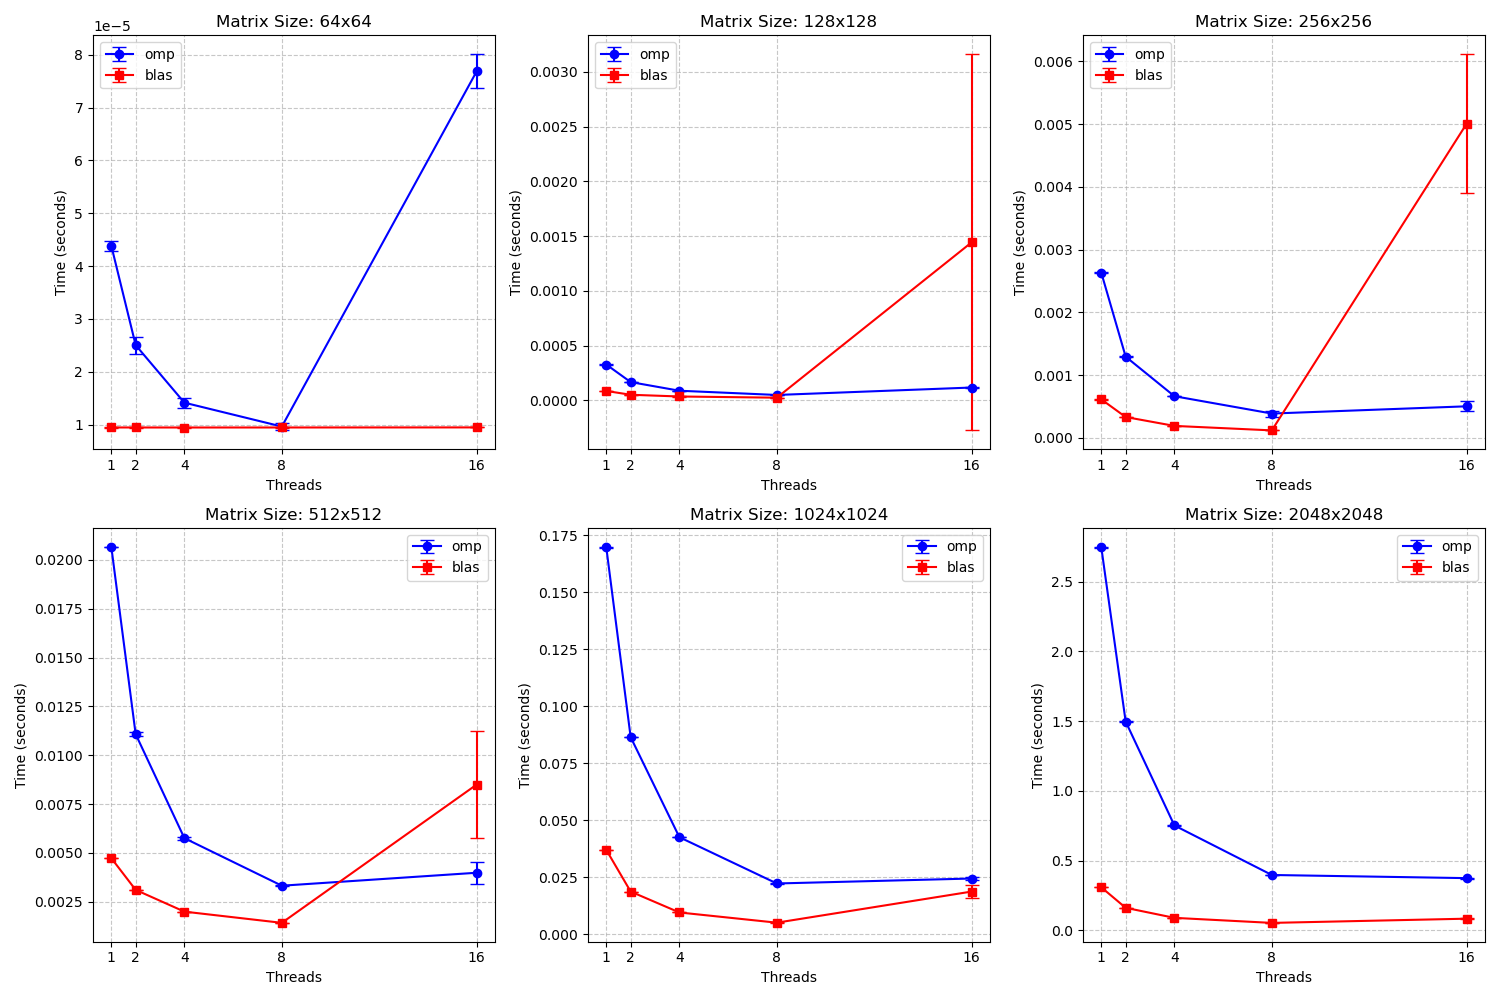
\includegraphics[width=0.9\textwidth]{Images/scaling_plot.png}
    \caption{Temps d'exécution en fonction du nombre de threads pour différentes tailles de matrices.}
    \label{fig:scaling_time}
\end{figure}

\begin{figure}[H]
    \centering
    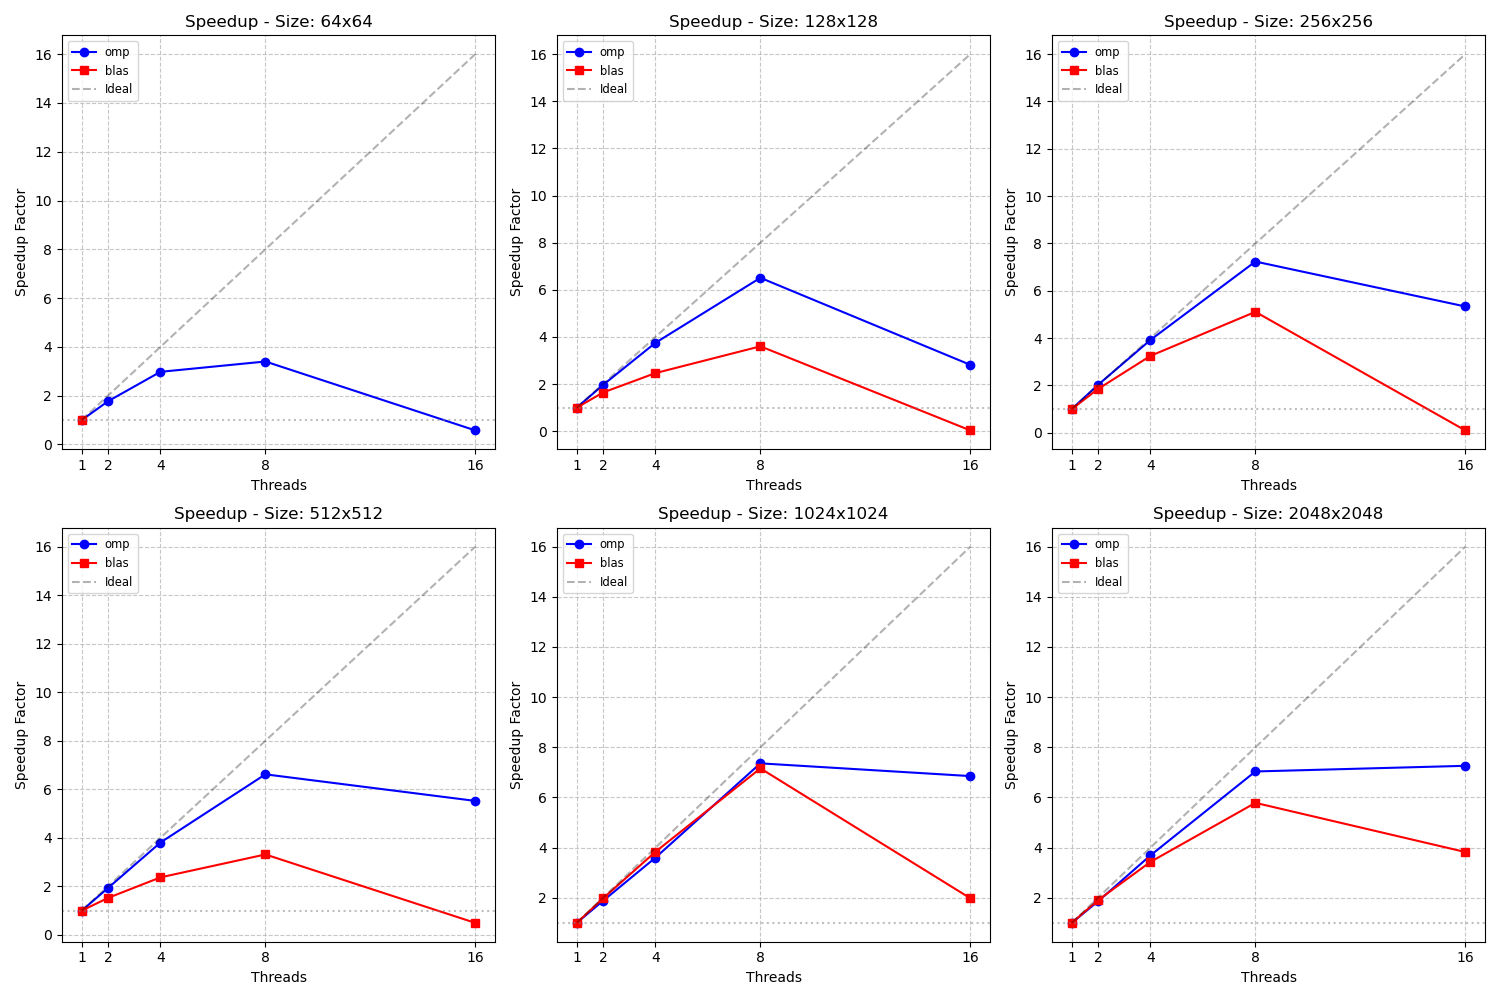
\includegraphics[width=0.9\textwidth]{Images/scaling_speedup_plot.png}
    \caption{Speedup (accélération) en fonction du nombre de threads.}
    \label{fig:scaling_speedup}
\end{figure}

\paragraph{Analyse des petites matrices ($N = 64 \times 64$).}
La parallélisation OpenMP apporte un gain conforme aux attentes entre 2 et 8 threads, mais devient contre-productive au-delà de 8 threads (au-delà du nombre de cœurs physiques). À cette échelle, la granularité du calcul est trop fine : la charge utile par thread devient comparable, voire inférieure, au surcoût de gestion (création, synchronisation et contention des ressources), ce qui annule les gains, voire dégrade les performances.

À l'inverse, BLAS reste monothread sur des matrices $64 \times 64$, la charge de calcul n'atteignant pas son seuil interne de déclenchement du parallélisme. Ainsi, pour cette échelle, les configurations les plus efficaces consistent soit à utiliser BLAS, soit à recourir à OpenMP en limitant le nombre de threads au nombre de cœurs physiques (8 threads dans notre cas).

\paragraph{Matrices de taille intermédiaire ($128 \times 128$ à $1024 \times 1024$).}
Pour les matrices de taille intermédiaire, OpenMP présente une accélération nette lorsque le nombre de threads augmente jusqu'au nombre de cœurs physiques disponibles. Au-delà de ce seuil, les gains se tassent, voire deviennent négatifs, sous l'effet de la saturation des ressources partagées et de l'augmentation des coûts de synchronisation.

BLAS offre de meilleures performances globales grâce à ses optimisations internes (vectorisation et découpage en blocs). Cependant, lorsque le nombre de threads dépasse le nombre de cœurs physiques, ses performances se dégradent et deviennent instables, principalement en raison de la contention des ressources et des changements de contexte (\emph{context switching}) sur un même cœur.

\paragraph{Grandes matrices ($2048 \times 2048$).}
Pour les matrices de grande taille, les deux approches bénéficient d'une parallélisation efficace jusqu'à environ 8 threads. Toutefois, l'augmentation du nombre de threads au-delà de ce point n'entraîne plus de gain significatif, le calcul devenant principalement limité par la bande passante mémoire. Dans ce contexte, BLAS reste la solution la plus performante et la plus stable.

Ainsi, l'efficacité du parallélisme dépend non seulement de la taille du problème, mais aussi d'une adéquation stricte entre nombre de threads et ressources matérielles disponibles.

\subsubsection{Hiérarchie des performances et Speedup}

La comparaison globale des implémentations sur grandes matrices met en évidence cinq paliers de performance (Figure~\ref{fig:comparison}) :

\begin{figure}[H]
    \centering
    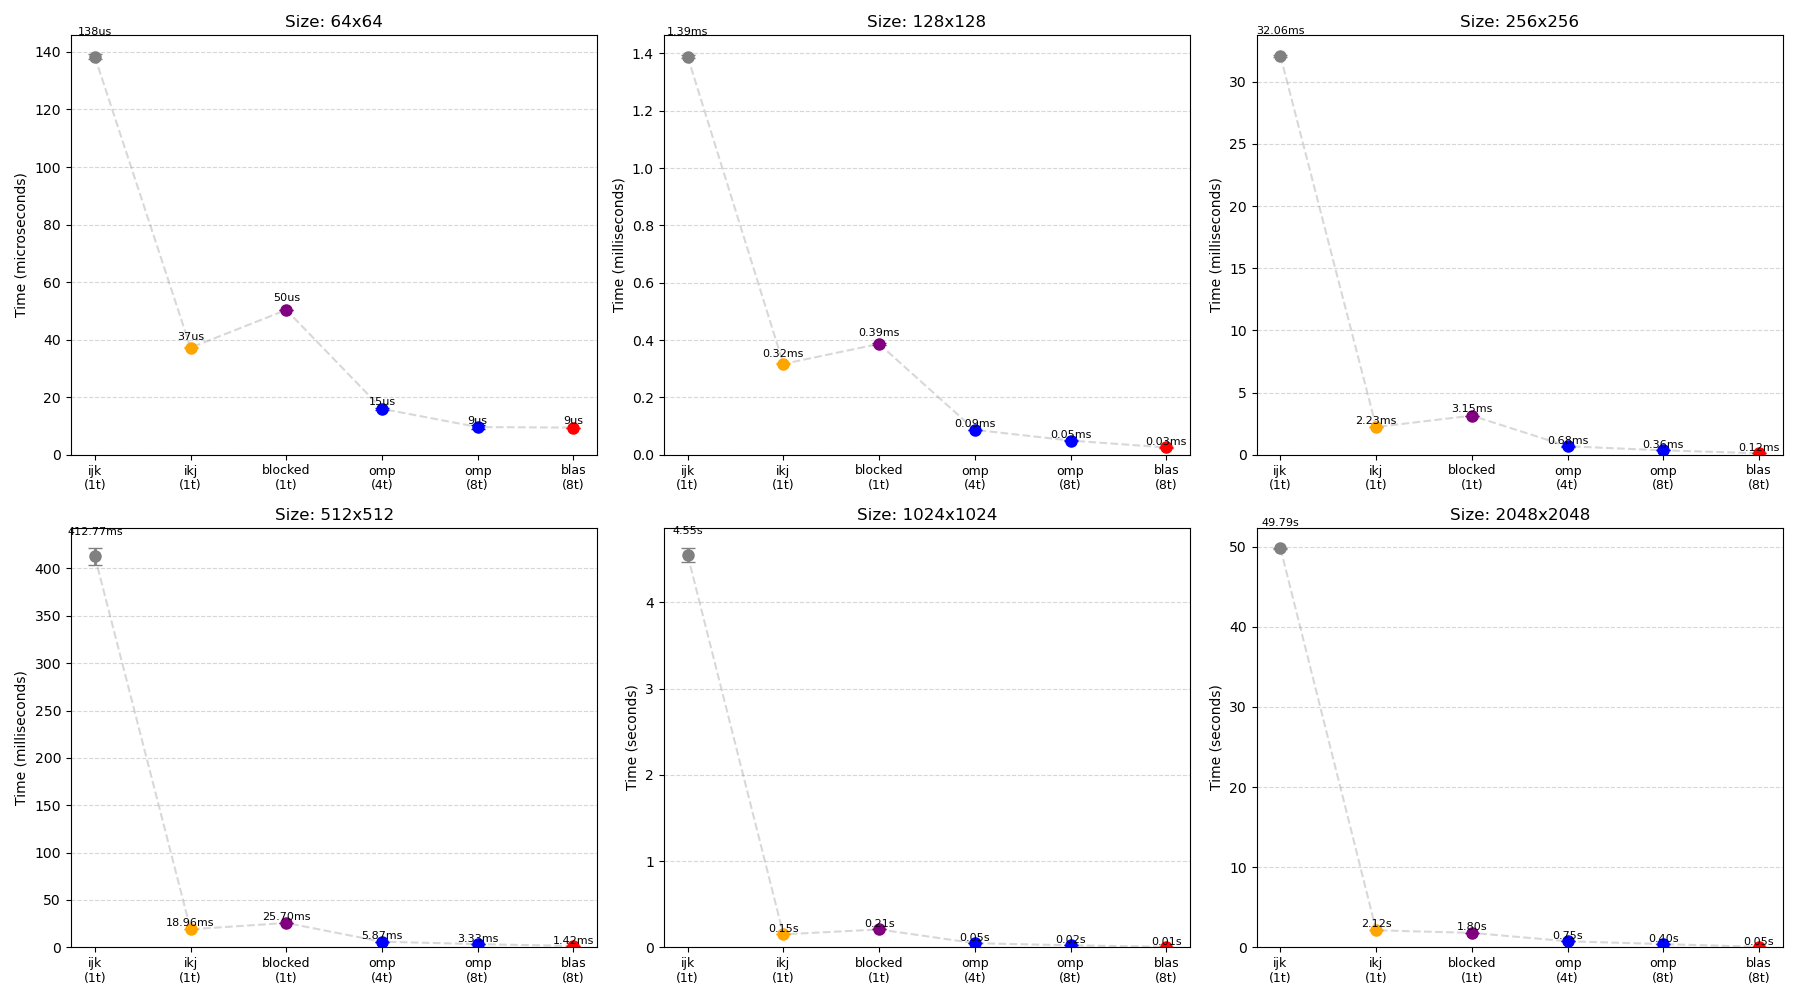
\includegraphics[width=1.0\textwidth]{Images/comparison_grid_plot.png}
    \caption{Comparaison des temps d'exécution (Naïf vs Reordered vs OpenMP vs BLAS).}
    \label{fig:comparison}
\end{figure}

\begin{figure}[H]
    \centering
    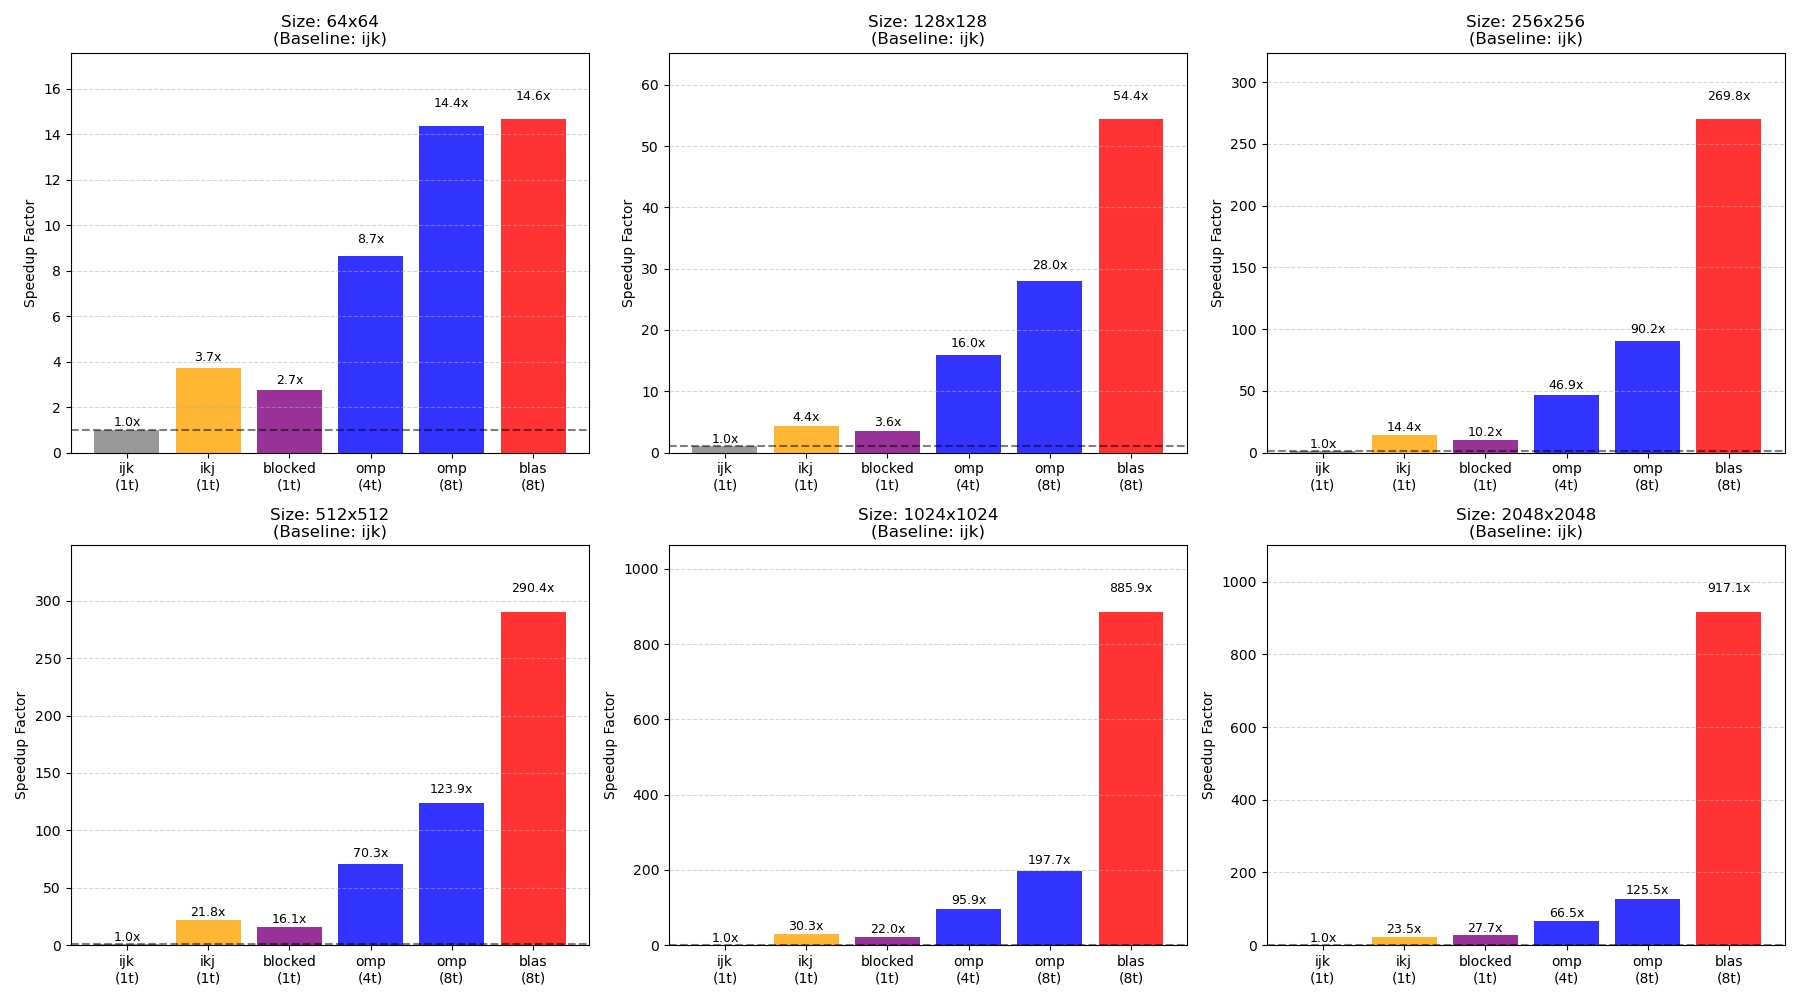
\includegraphics[width=1.0\textwidth]{Images/comparison_speedup_grid.png}
    \caption{Speedup relatif des différentes optimisations.}
    \label{fig:comparison_speedup}
\end{figure}

\begin{enumerate}
    \item \textbf{Naïf ($ijk$)} : L'ordre des boucles induit un parcours mémoire très défavorable, entraînant de nombreuses fautes de cache. Le temps d'exécution devient prohibitif pour les grandes tailles, atteignant plusieurs secondes pour $N=2048$.
    
    \item \textbf{Réordonné ($ikj$)} : La permutation des boucles améliore la localité spatiale des accès mémoire et permet un premier gain significatif par rapport à l'implémentation naïve, en particulier pour les tailles intermédiaires et grandes.
    
    \item \textbf{Bloqué (blocked)} : Cette optimisation apporte un gain mesurable par rapport à la version réordonnée, en améliorant la réutilisation des données dans les caches.
    
    \item \textbf{OpenMP} : La parallélisation sur 8 cœurs permet d'exploiter le parallélisme matériel et apporte un gain supplémentaire, bien que celui-ci reste contraint par le nombre de cœurs physiques et par la hiérarchie mémoire.
    
    \item \textbf{BLAS (OpenBLAS)} : Grâce à la combinaison d'optimisations avancées — blocage hiérarchique, vectorisation (AVX2/FMA) et micro-noyaux optimisés — BLAS surpasse largement les implémentations manuelles, avec un speedup pouvant atteindre plusieurs centaines de fois par rapport à la version naïve pour les plus grandes tailles.
\end{enumerate}

\subsubsection{Analyse de Profiling et Loi d'Amdahl : vers l'entraînement complet}

Afin de comprendre l'impact de ces optimisations sur le temps total d'apprentissage, nous avons profilé une époque complète d'entraînement (forward + backward) avec \texttt{gprof}.

\begin{tabular}{@{}ll@{}}
\textbf{Architecture} & : MLP 784 $\to$ 128 $\to$ 10 avec ReLU \\
\textbf{Taille du mini-batch} & : 64 \\
\textbf{Données}      & : MNIST Train (60 000 images)
\end{tabular}

\textbf{Avant optimisation (Kernel Naïf) :}
L'application est totalement limitée par le calcul (\emph{compute-bound}). La fonction \texttt{Matrix::matmul} consomme \textbf{environ 96\%} du temps total (Tableau~\ref{tab:gprof_naive}).

\begin{table}[H]
    \centering
    \caption{Profil d'exécution (gprof) - Version Naïve : \texttt{Matrix::matmul} domine (96.4\%)}
    \label{tab:gprof_naive}
    \begin{tabular}{lccl}
        \toprule
        \textbf{\% Time} & \textbf{Self (s)} & \textbf{Calls} & \textbf{Function Name} \\
        \midrule
        96.42 & 11.84 & 6256 & \texttt{Matrix::matmul} \\
        1.06 & 0.13 & 1252 & \texttt{DataLoader::nextBatch} \\
        0.73 & 0.09 & 3752 & \texttt{Matrix::transpose} \\
        0.41 & 0.05 & 12216 & \texttt{Matrix::Matrix (constructor)} \\
        0.24 & 0.03 & 95M & \texttt{Matrix::operator() const} \\
        0.24 & 0.03 & 74M & \texttt{Matrix::operator() (mut)} \\
        0.24 & 0.03 & 9380 & \texttt{Node::addGrad} \\
        0.24 & 0.03 & 1 & \texttt{MNISTDataset::load} \\
        0.16 & 0.02 & - & \texttt{\_init} \\
        0.08 & 0.01 & 2504 & \texttt{MathOps::add} \\
        \bottomrule
    \end{tabular}
\end{table}

\textbf{Après optimisation (BLAS) :}
Le temps passé dans \texttt{Matrix::matmul} s'effondre à moins de \textbf{1\%} ($\approx 0.5$s). Le goulot d'étranglement se déplace alors vers :
\par\smallskip
\noindent\textbf{Chargement des données (\texttt{MNISTDataset::load}).} Il représente $\approx 43\%$ du temps. Ce coût élevé s'explique par l'allocation et l'initialisation à zéro (inhérente au constructeur \texttt{std::vector}) d'un volume important de mémoire (376 Mo), suivies d'une copie avec conversion de type (\texttt{uint8\_t} vers \texttt{double}) pour chaque pixel.
\par\smallskip
\noindent\textbf{Allocations mémoire (\texttt{Matrix::Matrix}).} Elles représentent $\approx 29\%$ du temps.

\begin{table}[H]
    \centering
    \caption{Profil d'exécution (gprof) - Version BLAS : \texttt{matmul} négligeable, overhead mémoire dominant}
    \label{tab:gprof_blas}
    \begin{tabular}{lccl}
        \toprule
        \textbf{\% Time} & \textbf{Self (s)} & \textbf{Calls} & \textbf{Function Name} \\
        \midrule
        42.86 & 0.03 & 1 & \texttt{MNISTDataset::load} \\
        28.57 & 0.02 & 12216 & \texttt{Matrix::Matrix (init double)} \\
        28.57 & 0.02 & 938 & \texttt{SGDOptimizer::step} \\
        0.00 & 0.00 & 6256 & \texttt{Matrix::matmul} (optimisé par BLAS) \\
        0.00 & 0.00 & 95M & \texttt{Matrix::operator() const} \\
        0.00 & 0.00 & 74M & \texttt{Matrix::operator() (mut)} \\
        0.00 & 0.00 & 40k & \texttt{std::mersenne\_twister} \\
        0.00 & 0.00 & 18k & \texttt{Matrix::Matrix (copy)} \\
        0.00 & 0.00 & 10k & \texttt{std::\_Hashtable...} \\
        0.00 & 0.00 & 10k & \texttt{Node::Node} \\
        \bottomrule
    \end{tabular}
\end{table}

\textbf{Conséquence (Loi d'Amdahl) :}
Bien que le noyau de calcul soit accéléré de plusieurs centaines de fois au niveau micro-benchmark, l'accélération \textit{end-to-end} reste limitée par le chargement des données et les allocations mémoire. Dans nos mesures, une époque passe de 13.27s à 1.74s, soit un \textbf{speedup de 7.6x}. Ce résultat illustre la loi d'Amdahl \cite{amdahl1967} : après optimisation de \texttt{matmul}, les gains supplémentaires nécessitent d'agir sur la gestion mémoire et les entrées/sorties.

\begin{figure}[H]
    \centering
    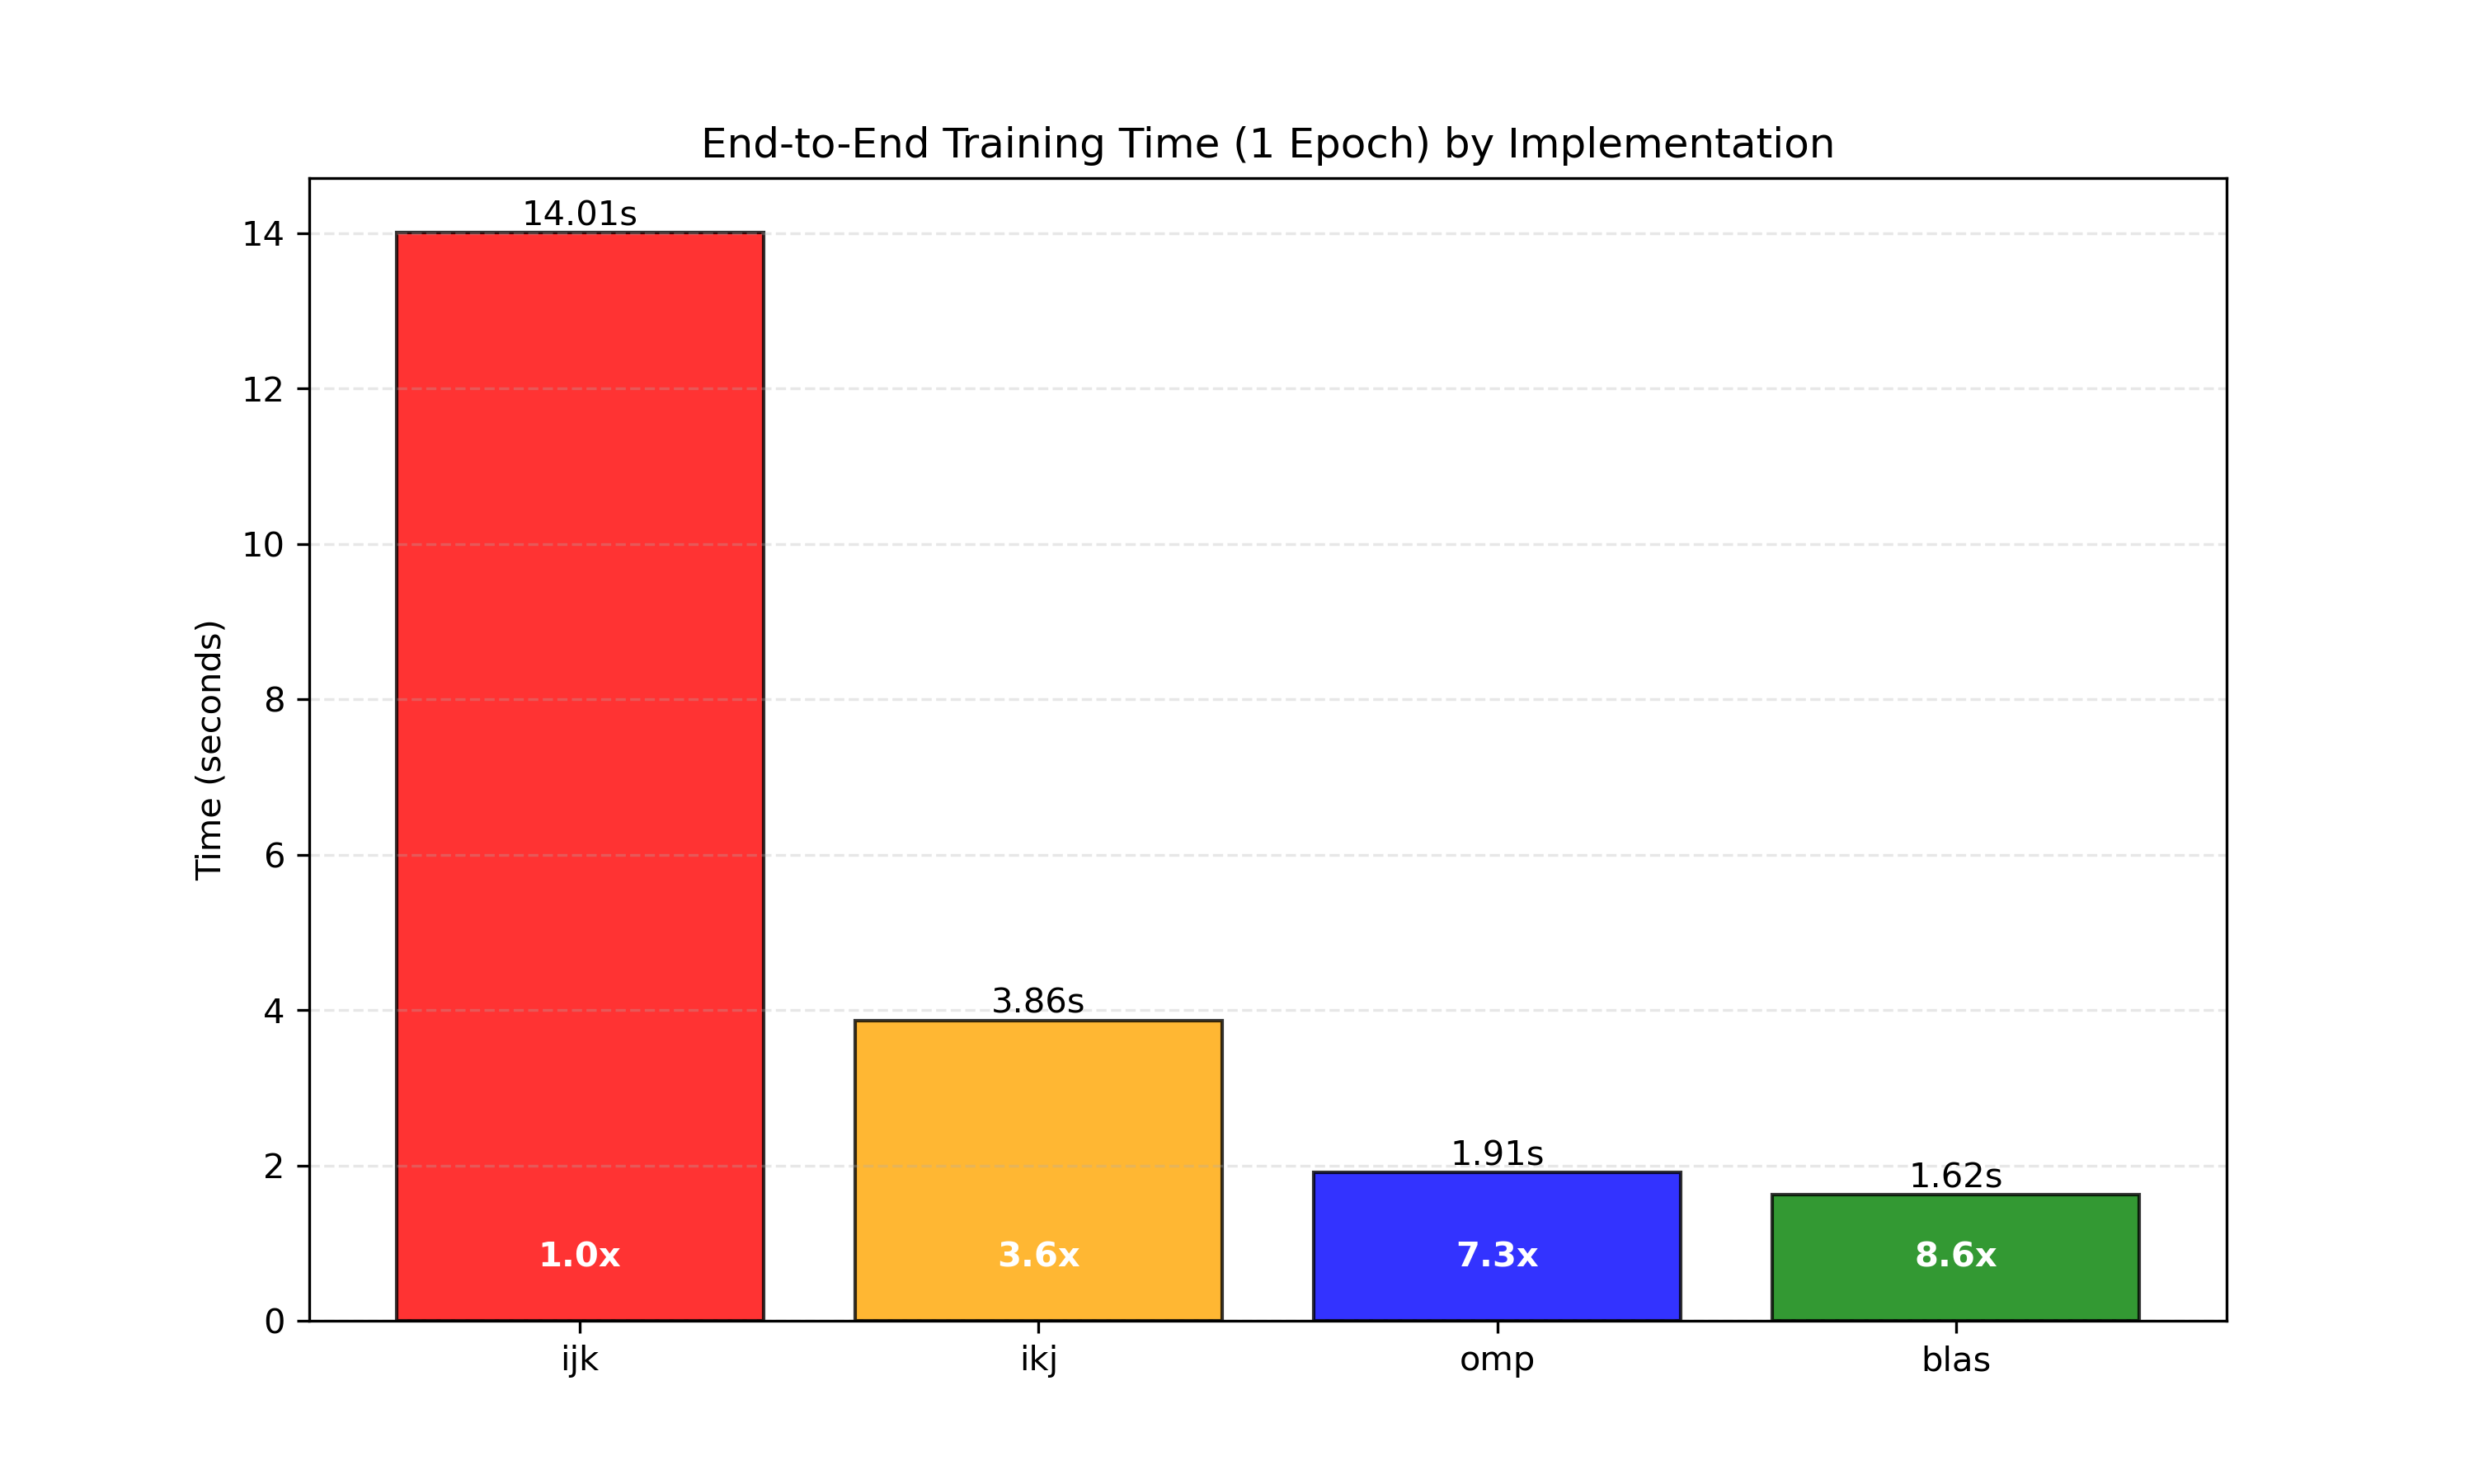
\includegraphics[width=0.8\textwidth]{Images/e2e_benchmark_plot.png}
    \caption{Répartition du temps d'exécution (End-to-End) : Naïf vs BLAS.}
    \label{fig:e2e_benchmark}
\end{figure}

\subsection{Convergence de l'entraînement}

\subsubsection{Premiers tests de convergence}

Afin de valider la correction du modèle et de l'algorithme d'optimisation, nous présentons la courbe d'apprentissage sur MNIST. L'ensemble des scripts et commandes utilisés pour reproduire ces expériences est disponible en Annexe~\ref{app:scripts}.

Les paramètres utilisés pour ce premier test sont :

\begin{table}[H]
    \centering
    \begin{tabular}{|l|l|}
        \hline
        \textbf{Paramètre} & \textbf{Valeur} \\
        \hline
        Taux d'apprentissage ($LR$) & $0.01$ \\
        Taille de batch ($B$) & $64$ \\
        Taille cachée ($H$) & $128$ \\
        Fonction d'activation & ReLU \\
        Initialisation & He \\
        Époques & $20$ \\
        \hline
    \end{tabular}
    \caption{Configuration standard pour le test de convergence.}
    \label{tab:convergence_config}
\end{table}

\begin{figure}[H]
    \centering
    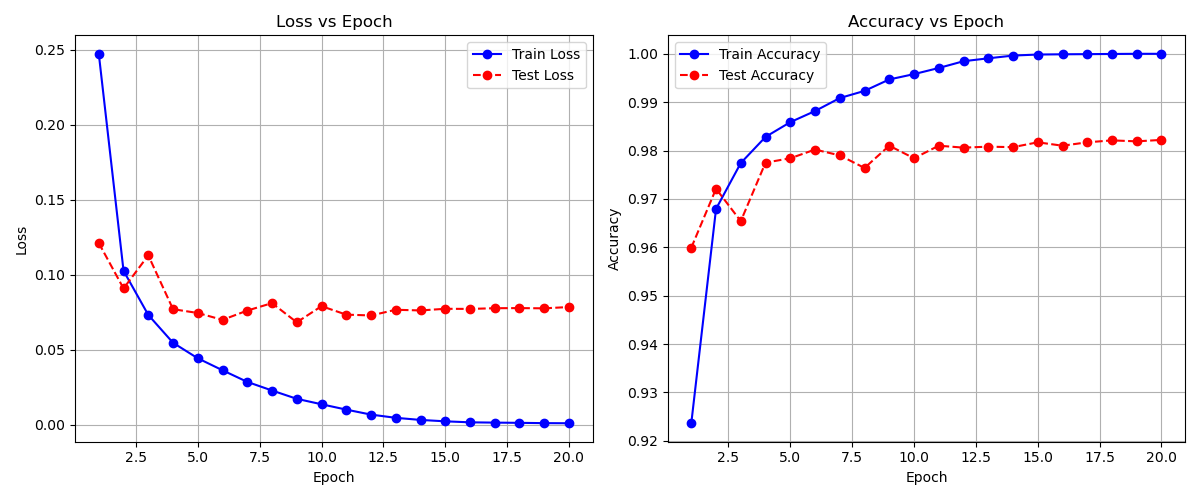
\includegraphics[width=0.8\textwidth]{Images/training_curve.png}
    \caption{Courbe de \textit{loss} et de précision (\textit{accuracy}) sur les données d'entraînement (\textbf{60 000 images}) et de validation (\textbf{10 000 images}).}
    \label{fig:training_curve}
\end{figure}

\textbf{Commentaire sur la convergence (Figure~\ref{fig:training_curve}) :}
Cette figure présente deux graphiques : la \textit{loss} (à gauche) et la précision (à droite).
\par\smallskip
\noindent\textbf{Courbe bleue (\textit{train}).} Performance sur les données d'entraînement, reflétant la capacité du modèle à s'ajuster aux données vues.
\par\smallskip
\noindent\textbf{Courbe rouge (\textit{validation}).} Performance sur les données de validation, jamais vues pendant l'entraînement.
\textbf{Interprétation :} La courbe rouge suit la bleue mais reste légèrement en retrait (\textit{loss} plus élevée, précision plus faible). C'est attendu : un modèle obtient généralement de meilleures performances sur les données d'entraînement que sur des données inédites. Si l'écart devenait très important, cela indiquerait un sur-apprentissage (\textit{overfitting}) ; ici, il reste modéré, suggérant une généralisation correcte.

\subsubsection{Impact du Taux d'Apprentissage (Learning Rate)}

Nous avons évalué l'impact du taux d'apprentissage sur la convergence du modèle en testant les valeurs $\{0.025, 0.01, 0.0075, 0.005, 0.001\}$. Les autres hyperparamètres ont été fixés : batch $B=64$, couche cachée $H=128$, activation ReLU et initialisation He. Pour assurer la robustesse statistique, chaque configuration a été exécutée trois fois avec des graines différentes.

La Figure~\ref{fig:lr_results} présente les résultats obtenus.

\begin{figure}[H]
    \centering
    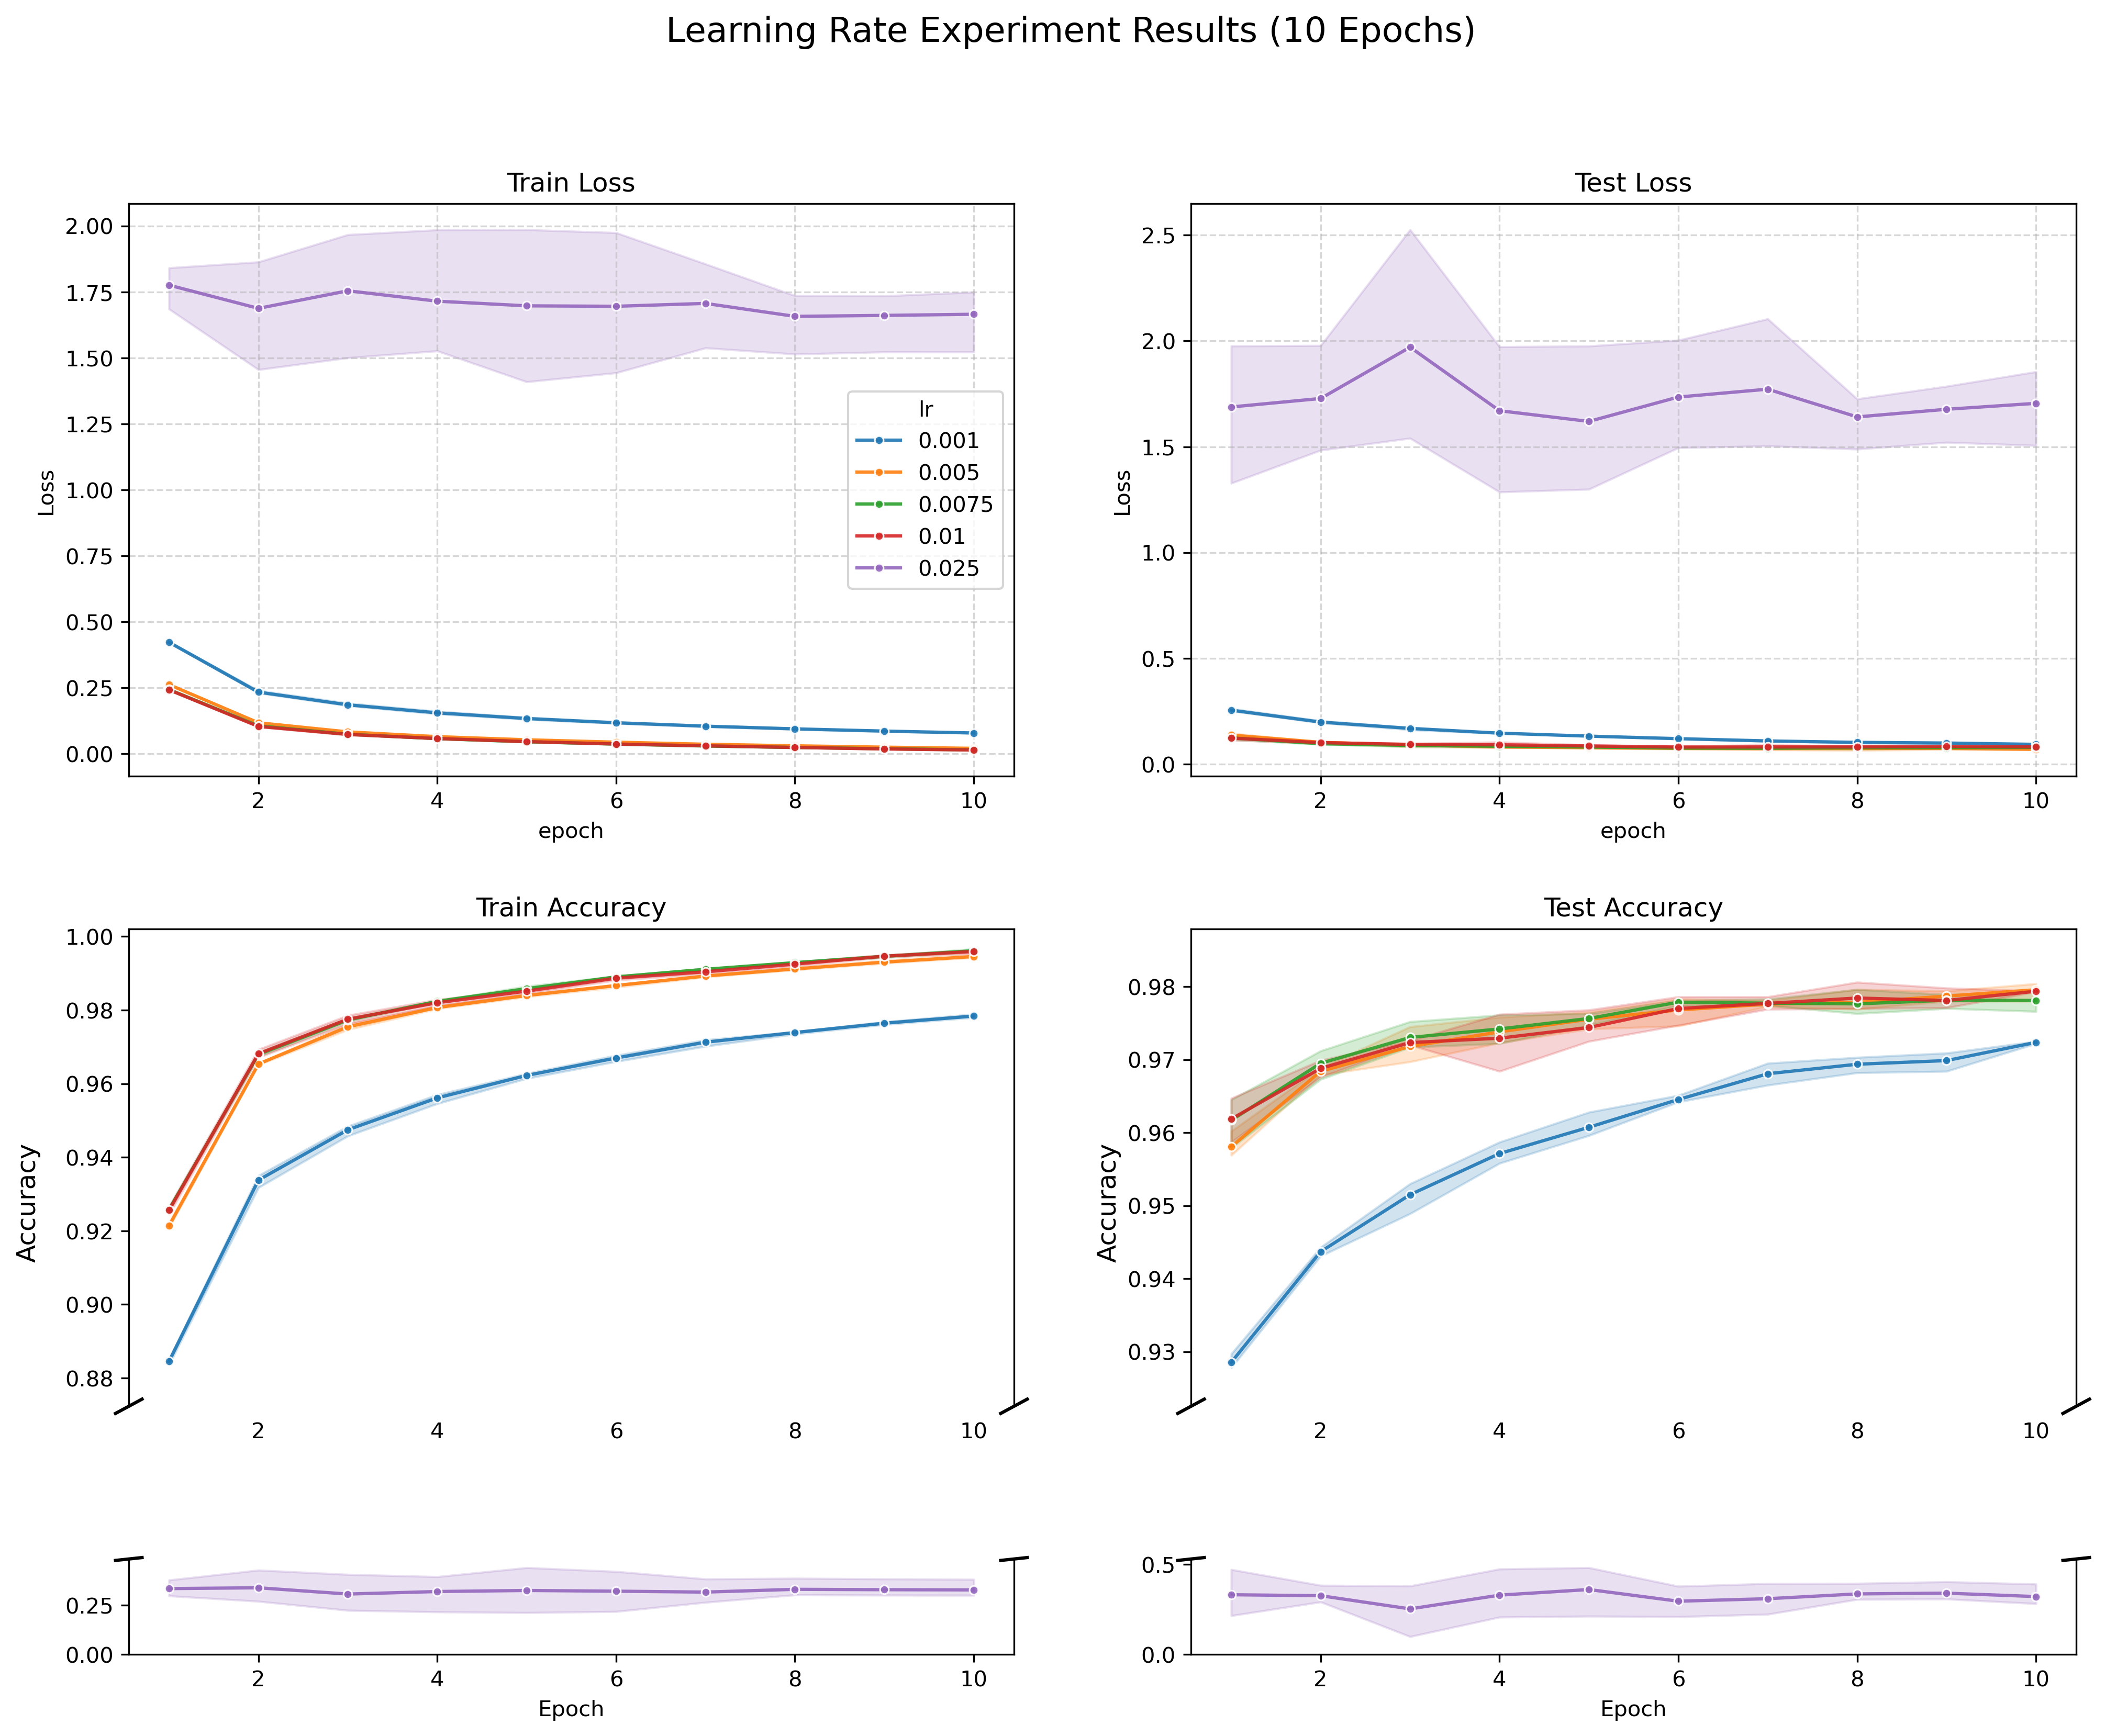
\includegraphics[width=1.0\textwidth]{Images/combined_lr_results.png}
    \caption{Impact du \textit{learning rate} sur la convergence (10 époques, 3 graines). Les axes de précision utilisent une échelle discontinue pour visualiser simultanément les hautes précisions ($>90\%$) et les échecs de convergence ($<40\%$).}
    \label{fig:lr_results}
\end{figure}

\par\smallskip
\noindent\textbf{Taux trop faible ($LR=0.001$).} Le modèle converge, mais trop lentement. Après 10 époques, la précision de validation plafonne à $\sim97.2\%$, inférieure à celle obtenue avec des taux plus élevés, car les mises à jour des poids sont trop petites pour atteindre l'optimum rapidement.
\par\smallskip
\noindent\textbf{Zone optimale ($LR \in [0.005, 0.01]$).} Ces taux offrent le meilleur compromis, avec une convergence rapide et stable, atteignant une précision de $\sim97.9\%$ à $\sim98.0\%$. Nous retenons $LR=0.01$ pour sa rapidité.
\par\smallskip
\noindent\textbf{Taux trop élevé ($LR=0.025$).} On observe une instabilité critique (divergence) : les pas de gradient sont trop grands et l'optimiseur franchit les minima de la \textit{loss}, conduisant à une précision d'environ $\sim32.1\%$ et à une variance élevée ($\sigma \approx 0.06$), rendant l'entraînement inefficace.

Ces résultats expérimentaux confirment directement les intuitions théoriques présentées en section \ref{sec:theory_sgd} concernant les risques de divergence (taux trop grand) et la lenteur de convergence (taux trop faible).

Nous retenons donc \textbf{$LR=0.01$} comme valeur optimale pour la suite.

\subsubsection{Impact de la Taille de Batch (Batch Size)}

En fixant $LR=0.01$, nous avons étudié l'impact de la taille de batch $\{16, 32, 64, 128, 256\}$ sur la stabilité et la performance.

La Figure~\ref{fig:batch_results} illustre ces résultats.

\begin{figure}[H]
    \centering
    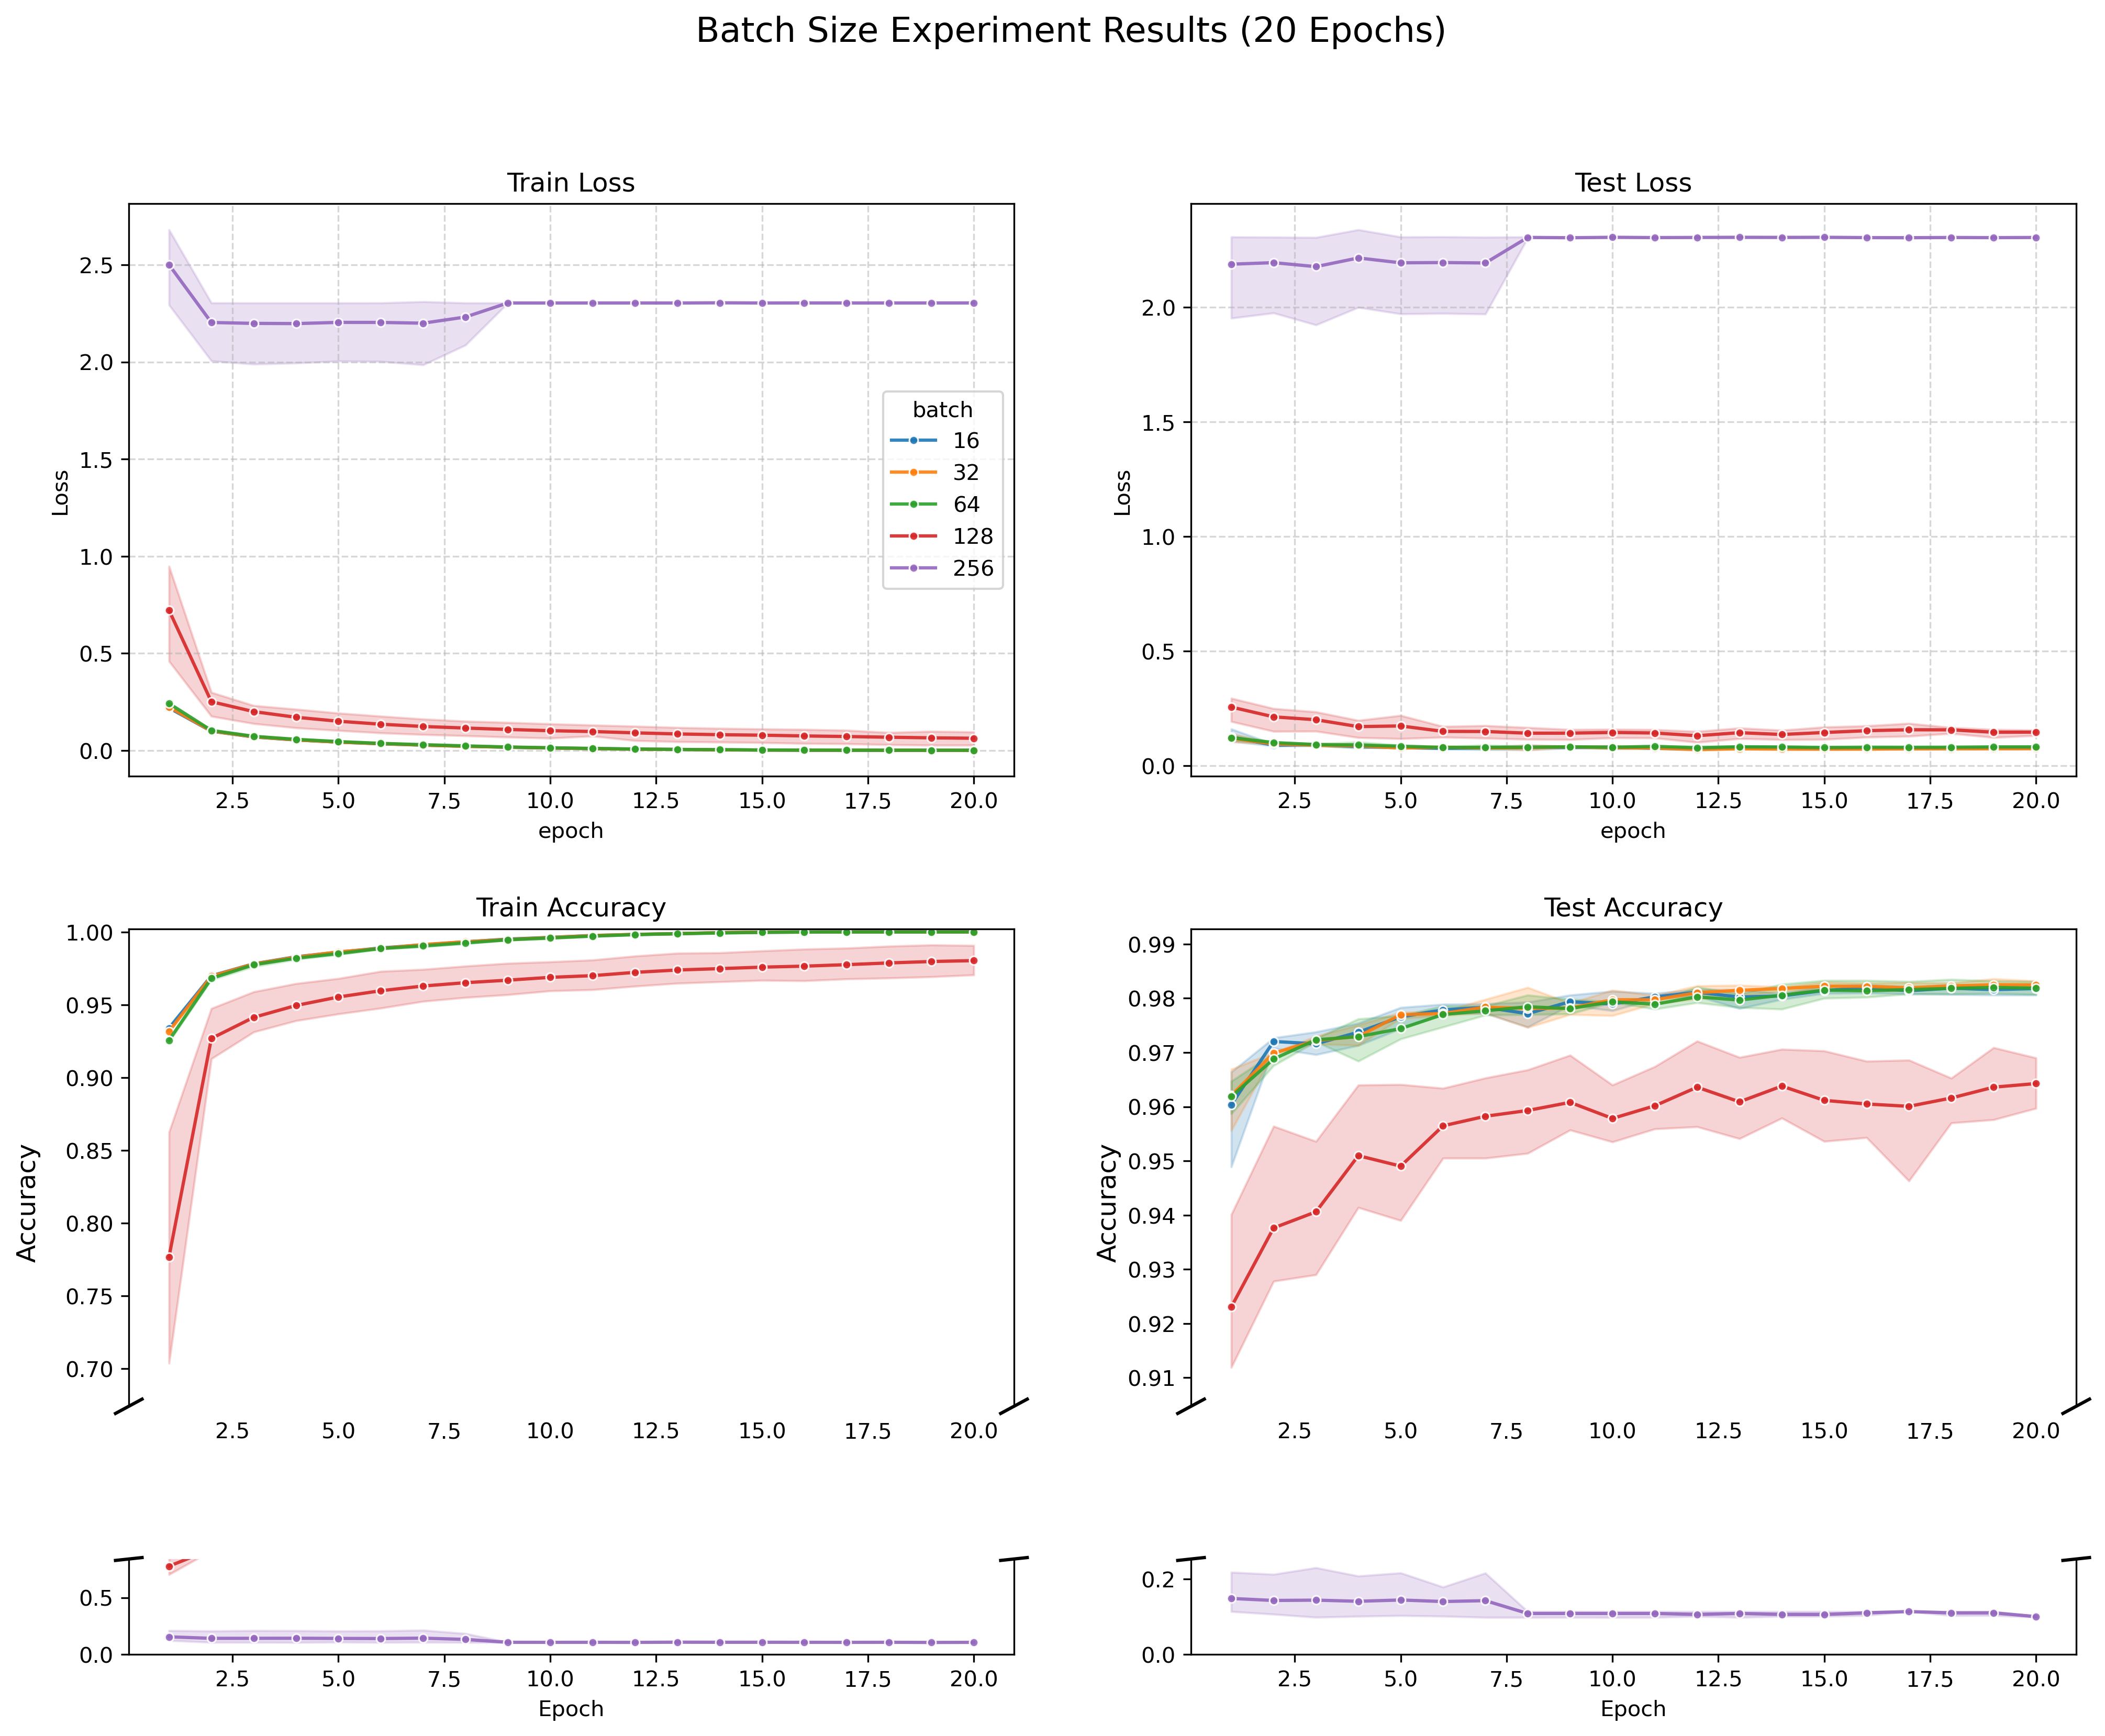
\includegraphics[width=1.0\textwidth]{Images/combined_batch_results.png}
    \caption{Impact de la Taille de Batch (20 époques, $LR=0.01$, 3 graines). Les petits batchs (16, 32) convergent mieux mais sont plus lents à exécuter. Le batch 256 diverge avec ce $LR$ fixe.}
    \label{fig:batch_results}
\end{figure}

\par\smallskip
\noindent\textbf{Petits batchs (16, 32).} Ils offrent la meilleure précision finale ($\sim98.2\%$), vraisemblablement grâce au bruit introduit dans l'estimation du gradient, qui peut favoriser la généralisation. Aucune différence significative n'est observée entre 16 et 32.
\par\smallskip
\noindent\textbf{Batch moyen (64).} Il constitue un compromis, avec une précision comparable ($\sim98.2\%$) et une meilleure efficacité de calcul (parallélisation plus importante).
\par\smallskip
\noindent\textbf{Grands batchs ($128, 256$).} La performance se dégrade avec $B=128$, et le modèle diverge avec $B=256$. Pour stabiliser $B=256$, il faudrait probablement ajuster le $LR$ (\textit{linear scaling rule}) ou utiliser un \textit{warm-up}, ce qui n'est pas le cas ici avec $LR=0.01$ fixe.

\textit{Note : Les grands batchs sont plus rapides à exécuter par époque, car les opérations matricielles plus larges exploitent mieux le parallélisme matériel (CPU/GPU) et la vectorisation. Les petits batchs génèrent davantage d'appels noyau (surcoût) et n'utilisent qu'une partie des unités de calcul, ce qui les rend plus lents malgré leur meilleure stabilité d'optimisation.}

\subsubsection{Impact de la Taille de la Couche Cachée (Hidden Size)}

Enfin, en fixant $LR=0.01$ et un batch $B=64$, nous avons évalué l'impact du nombre de neurones dans la couche cachée $\{64, 128, 256\}$ sur la capacité du modèle.

La Figure~\ref{fig:hidden_results} illustre ces résultats.

\begin{figure}[H]
    \centering
    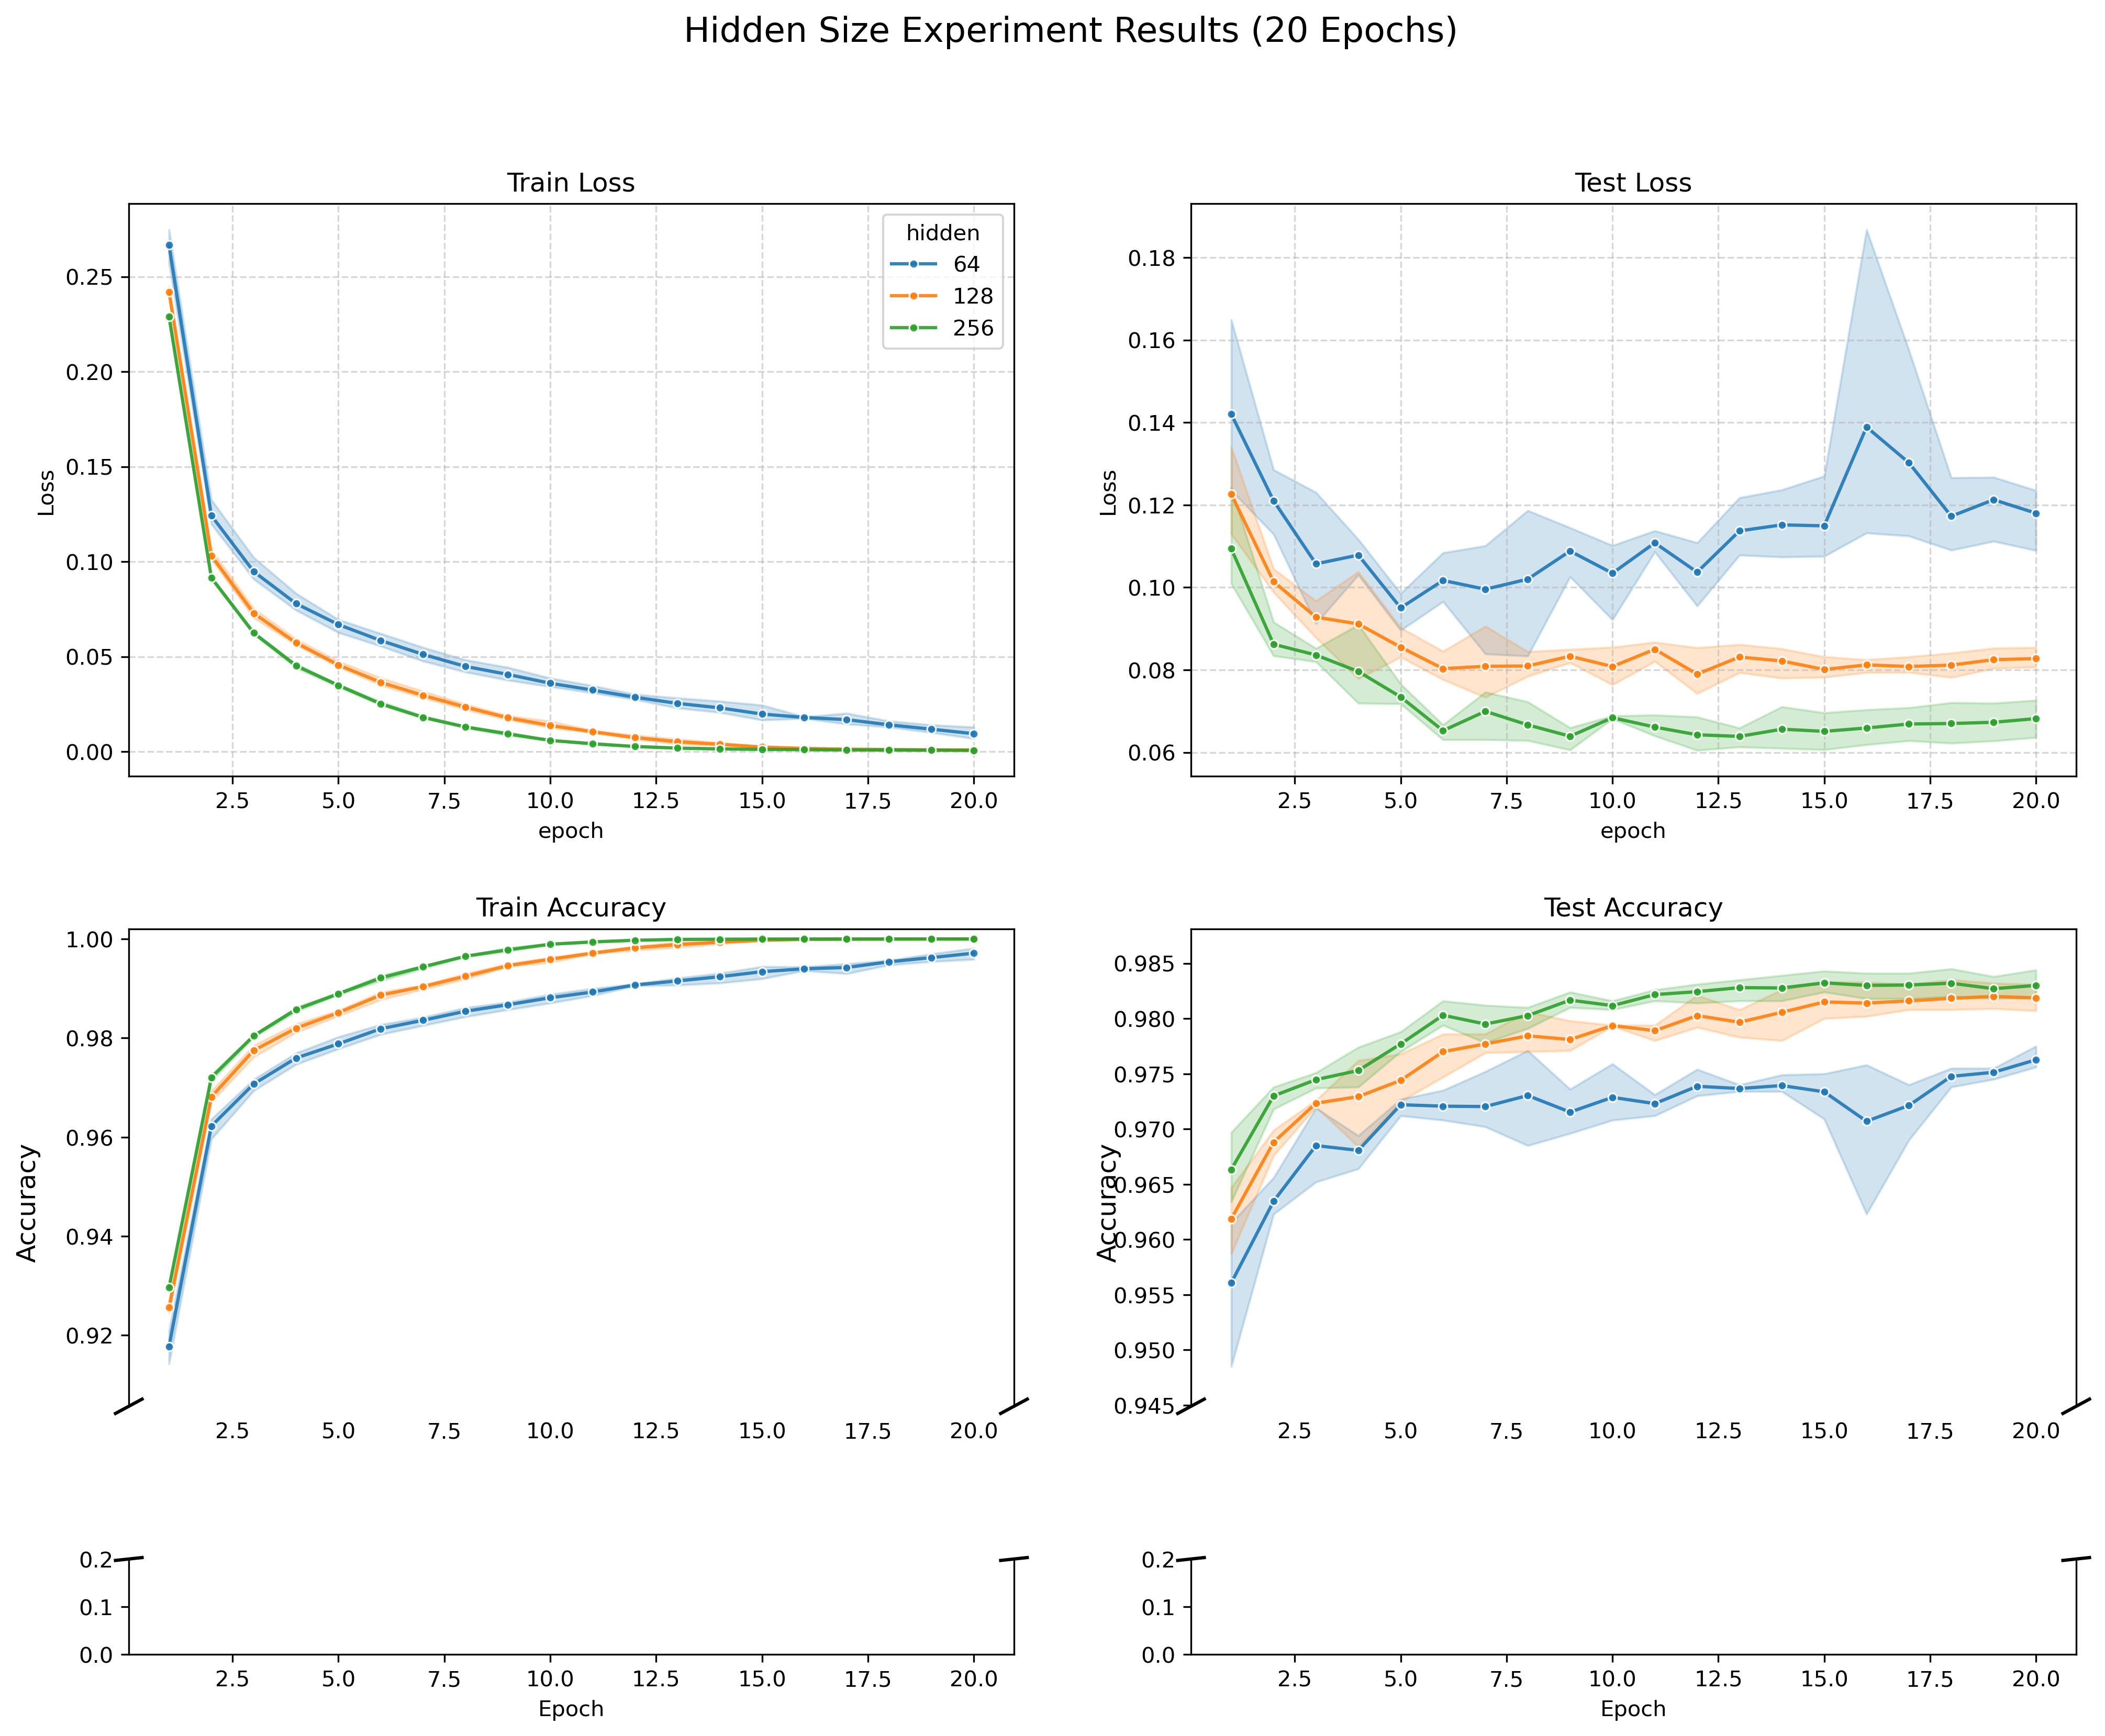
\includegraphics[width=1.0\textwidth]{Images/combined_hidden_results.png}
    \caption{Impact de la Taille de la Couche Cachée (20 époques, $LR=0.01, B=64$, 3 graines). L'augmentation de la taille améliore la précision, mais avec des rendements décroissants au-delà de 128 neurones.}
    \label{fig:hidden_results}
\end{figure}

\par\smallskip
\noindent\textbf{Capacité limitée ($H=64$).} Le modèle sous-apprend légèrement, avec une précision d'environ $\sim97.6\%$. Cela suggère que 64 neurones ne suffisent pas à capturer toute la complexité de MNIST avec cette architecture.
\par\smallskip
\noindent\textbf{Compromis ($H=128$).} La précision atteint $\sim98.2\%$, avec un gain significatif par rapport à $H=64$ sans accroître excessivement le coût de calcul.
\par\smallskip
\noindent\textbf{Rendements décroissants ($H=256$).} La meilleure précision est obtenue ($\sim98.3\%$), mais le gain ($\approx 0.1\%$) reste marginal au regard du doublement du coût de calcul. Pour cette tâche, $H=128$ apparaît suffisant.

\subsubsection{Impact de la Fonction d'Activation et de l'Initialisation}

Nous avons comparé les fonctions d'activation \texttt{ReLU}, \texttt{Sigmoid} et \texttt{Tanh} (avec $LR=0.01, Batch=64, H=128$). Pour garantir une comparaison équitable, nous avons utilisé l'initialisation de \textbf{He} pour ReLU et de \textbf{Xavier} pour Sigmoid/Tanh. De plus, nous avons inclus une initialisation dite "Manuelle" (\textit{Manual Init}), correspondant à une distribution uniforme simple $\mathcal{U} \sim [-0.1, 0.1]$. Cette méthode naïve sert de point de référence (baseline) pour évaluer l'efficacité des méthodes modernes.

La Figure~\ref{fig:activation_results} présente les courbes de convergence.

\begin{figure}[H]
    \centering
    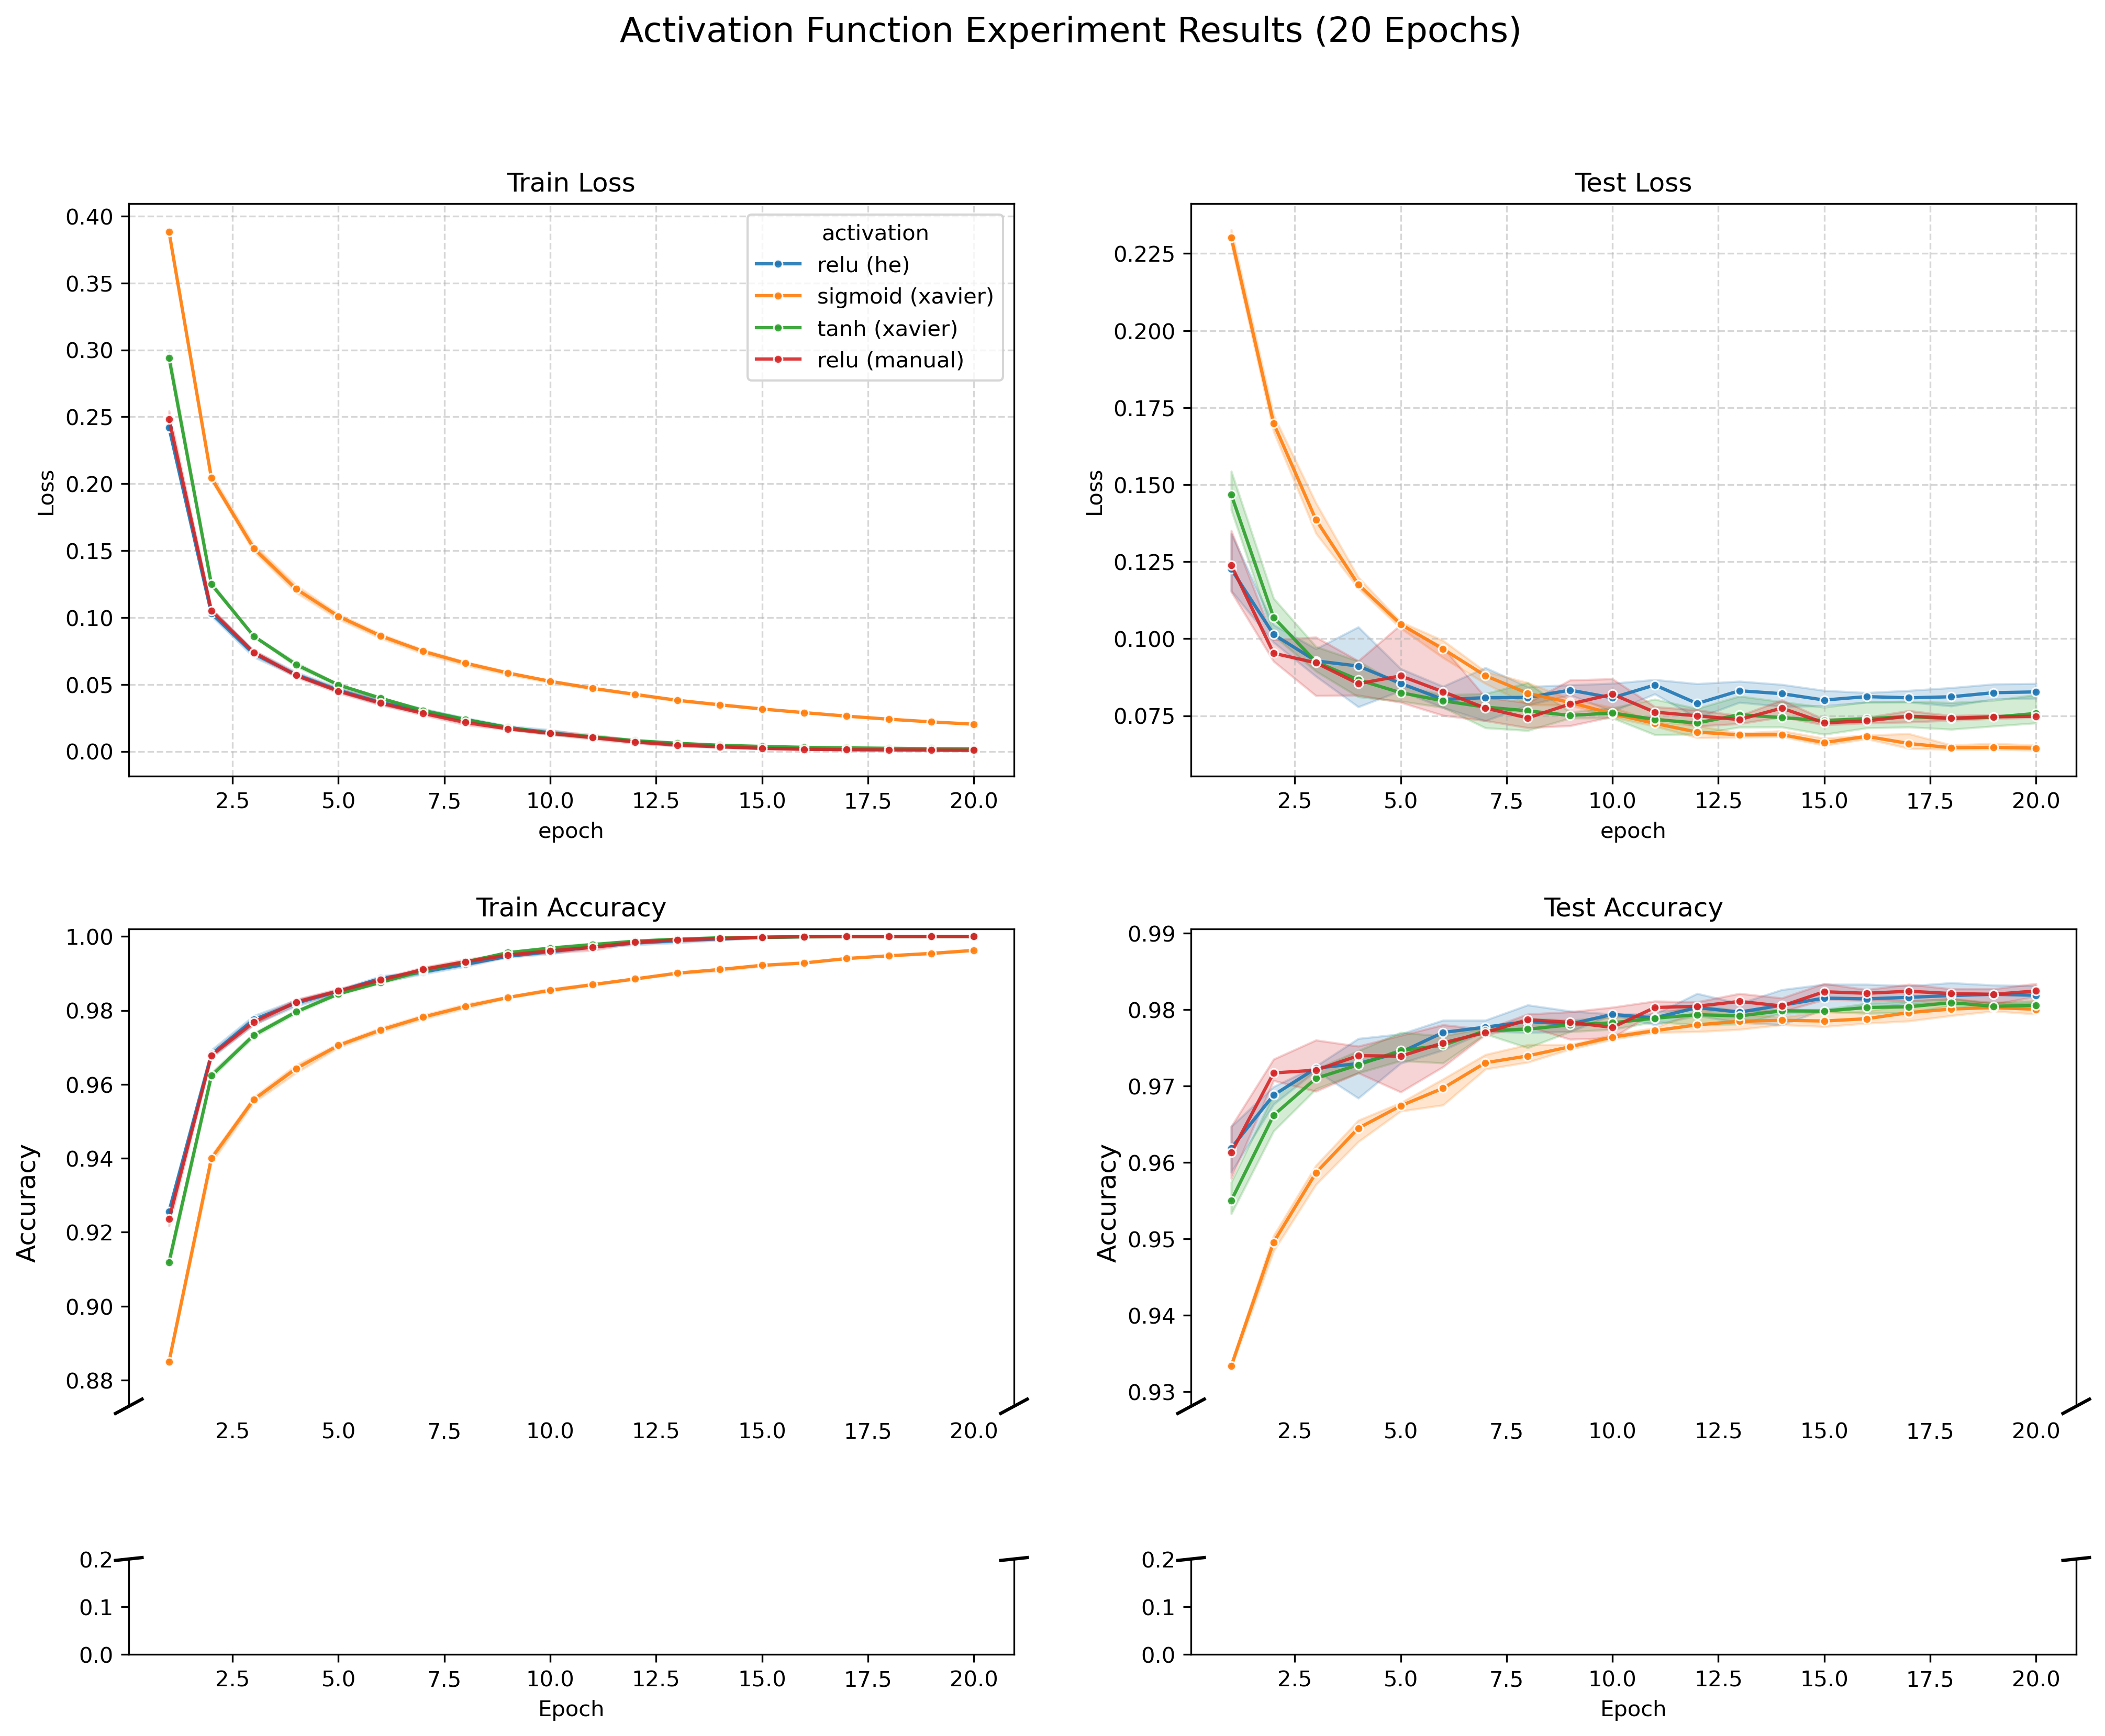
\includegraphics[width=1.0\textwidth]{Images/combined_activation_results.png}
    \caption{Comparaison des Fonctions d'Activation et Initialisation. ReLU (He) et ReLU (Manual) offrent les meilleures performances. Sigmoid et Tanh (avec Xavier) restent compétitifs grâce à une initialisation adaptée.}
    \label{fig:activation_results}
\end{figure}

\textbf{Analyse des performances (précision de validation moyenne) :}
\par\smallskip
\noindent\textbf{ReLU (Manual Init) [$\sim98.24\%$].} Notre initialisation manuelle $[-0.1, 0.1]$ obtient une performance comparable à l'initialisation de He. Cela s'explique par le fait que, pour $N_{in}=784$, l'écart-type de cette distribution uniforme ($\sim0.057$) est proche de l'optimum théorique de He ($\sim0.05$).
\par\smallskip
\noindent\textbf{ReLU (He Init) [$\sim98.19\%$].} La performance est quasi-identique à l'initialisation manuelle, confirmant la robustesse de ReLU sur ce problème.
\par\smallskip
\noindent\textbf{Tanh (Xavier) [$\sim98.06\%$] et Sigmoid (Xavier) [$\sim98.00\%$].} Bien que légèrement inférieures à ReLU, ces activations restent compétitives ici car l'initialisation de Xavier limite la saturation des gradients au début de l'entraînement. Sans cette initialisation, la convergence aurait été sensiblement dégradée.

\textbf{Synthèse théorique :}
\par\smallskip
\noindent\textbf{ReLU.} Standard actuel pour les \textbf{couches cachées} des réseaux profonds (CNN, MLP) : elle atténue le problème de disparition du gradient et reste très rapide à calculer.
\par\smallskip
\noindent\textbf{Sigmoid.} Principalement utilisée en \textbf{sortie} pour la classification binaire (probabilité $p \in [0,1]$). Elle est généralement à éviter dans les couches cachées profondes en raison de sa saturation (gradient $\to 0$).
\par\smallskip
\noindent\textbf{Tanh.} Souvent préférée à Sigmoid dans les couches cachées lorsque l'on souhaite des sorties centrées sur 0 (utile notamment pour certains RNN), mais elle souffre également de saturation.

\textbf{Conclusion finale des expériences :}
La configuration optimale retenue est : \textbf{$LR=0.01$, $B=64$, $H=128$, activation ReLU, init. He/Manual}.

\subsubsection{Impact de l'Affinité sur les charges d'entrée (Input Layer)}

Les résultats présentés dans cette section analysent l'impact de l'affinité sur les opérations typiques de la couche d'entrée avec une taille de batch $B=64$ (soit une multiplication $64 \times 784 \times 128$, charge de travail comparable à une matrice carrée intermédiaire). Le tableau ci-dessous détaille les résultats pour 2 et 8 threads.

\begin{table}[H]
    \centering
    \caption{Impact de l'affinité sur les performances pour une multiplication matricielle $64 \times 784 \times 128$.}
    \label{tab:affinity}
    \begin{tabular}{llccc}
        \toprule
        \textbf{Threads} & \textbf{Affinité} & \textbf{Temps OMP ($\mu$s)} & \textbf{Temps BLAS ($\mu$s)} & \textbf{Ratio OMP/BLAS} \\
        \midrule
        2 & \texttt{default} & 480 & 132 & 3.6x \\
        2 & \texttt{close} & 474 & 128 & 3.7x \\
        2 & \texttt{spread} & 487 & 159 & 3.1x \\
        \midrule
        8 & \texttt{default} & 149 & 68 & 2.2x \\
        8 & \texttt{close} & 152 & 45 & 3.4x \\
        8 & \texttt{spread} & 236 & 75 & 3.1x \\
        \bottomrule
    \end{tabular}
\end{table}

L'analyse de ces données pour une multiplication $64 \times 784 \times 128$ révèle :
\par\smallskip
\noindent\textbf{Impact de l'affinité sur BLAS.} Le mode \texttt{close} est déterminant : à 8 threads, il réduit le temps à $45 \mu$s, contre $68 \mu$s en configuration \texttt{default}, soit un gain d'environ \textbf{33\%}. Le mode \texttt{spread} est le moins performant ($75 \mu$s), car il disperse les threads et pénalise la localité des caches partagés.
\par\smallskip
\noindent\textbf{Impact sur OpenMP.} Notre implémentation réagit différemment : à 8 threads, \texttt{default} ($149 \mu$s) et \texttt{close} ($152 \mu$s) sont comparables, tandis que \texttt{spread} dégrade fortement les performances ($236 \mu$s). Cela suggère que le placement par défaut est déjà relativement compact, et que forcer la dispersion nuit à la cohérence de cache de notre algorithme.

\textbf{Conclusion :} Pour les opérations de la couche d'entrée ($64 \times 784 \times 128$), l'utilisation de bibliothèques optimisées comme BLAS est impérative. Cependant, ces bibliothèques sont très sensibles à la localité : pour obtenir le gain de performance maximal (facteur $\times 4$ face à OpenMP), il est crucial de configurer l'affinité des threads (mode \texttt{close}) afin de minimiser les latences cache.

\subsection{Synthèse des Résultats Expérimentaux}
L'ensemble de ces expérimentations met en lumière la dualité du défi posé par les réseaux de neurones : un défi \textbf{algorithmique} (trouver les bons hyperparamètres pour la convergence) et un défi \textbf{computationnel} (exécuter ces calculs efficacement).

\textbf{Aspect algorithmique :} La recherche par grille a permis d'isoler une configuration robuste (\textbf{LR=0.01, Batch=64, H=128, ReLU}) capable d'atteindre $\sim98.2\%$ de précision sur MNIST, validant notre implémentation de la rétropropagation.
\textbf{Aspect performance :} L'optimisation bas niveau s'avère critique. L'utilisation de bibliothèques vectorisées (BLAS) avec une affinité CPU contrôlée (\texttt{close}) offre des gains de performance considérables sur le noyau de calcul ; dans nos mesures, la configuration la plus efficace correspond à \textbf{8 threads} avec \texttt{OMP\_PROC\_BIND=close}. Cependant, l'accélération globale de l'apprentissage reste bornée par les coûts de gestion mémoire et de chargement de données (loi d'Amdahl), soulignant l'importance d'une optimisation holistique du système.

\section{Déroulé du Projet}
L'état de l'art a été rédigé conjointement par Jianye, Hao et Xiang, afin de présenter le contexte théorique du projet et les approches existantes en matière de réseaux de neurones et de classification sur MNIST. L'équipe a ensuite organisé son travail en plusieurs phases successives, chacune portée par un ou plusieurs membres selon leurs affinités techniques.

La phase de conception a été initiée par Jianye, qui a rédigé la documentation préliminaire et produit la première version du diagramme UML, permettant de clarifier l'architecture générale du projet. La mise en place du premier prototype fonctionnel du MLP a ensuite été assurée par Abdennour, qui a développé les modules fondamentaux liés aux tenseurs, aux couches linéaires et aux fonctions d'activation.

La réalisation du moteur de différenciation automatique a été répartie entre Hao et Xiang, chacun prenant en charge une partie des opérations nécessaires au calcul du graphe et des gradients. Par la suite, Jianye a intégré l'ensemble de ces composants, généré une seconde version du diagramme UML pour refléter les ajustements apportés, et affiné la conception en fonction des problèmes rencontrés.

Le développement du mécanisme d'entraînement a été amorcé par Xiang, tandis que Jianye et Hao ont poursuivi respectivement l'implémentation de l'optimiseur et des fonctions de \textit{loss}. L'intégration du jeu de données MNIST et la validation du pipeline complet ont été assurées par Jianye.

Jianye a également mené des tests de performance et des analyses de profilage afin d'optimiser l'ensemble du système, ainsi qu'une recherche expérimentale visant à identifier une configuration robuste des hyperparamètres.

Enfin, la rédaction du rapport a été réalisée collectivement.

\section{Conclusion \& perspectives}

\subsection{Conclusion :}
Ce projet a permis de démystifier le fonctionnement interne des réseaux de neurones profonds en implémentant, à partir de zéro (\textit{from scratch}), un moteur complet d'apprentissage en C++. L'architecture retenue, basée sur un graphe de calcul dynamique (DAG) et la différenciation automatique, a démontré la flexibilité du C++ moderne (pointeurs intelligents, polymorphisme) pour modéliser des concepts mathématiques abstraits tout en garantissant une gestion rigoureuse de la mémoire.

Sur le plan de la performance, l'analyse expérimentale a mis en évidence l'impact critique des optimisations bas niveau. Si le noyau de calcul (\texttt{matmul}) a bénéficié d'une accélération spectaculaire de plus de trois ordres de grandeur grâce à BLAS et OpenMP, l'accélération globale de l'application est restée plus modeste ($7.6\times$). Ce contraste illustre la loi d'Amdahl : une fois le calcul matriciel optimisé, le goulot d'étranglement se déplace inévitablement vers la gestion des données (\textit{I/O}) et les allocations mémoire.

\textbf{Limites et menaces à la validité :}
Les conclusions de performance dépendent d'un protocole de mesure contrôlé (verrouillage de fréquence, affinité CPU) et peuvent varier sur d'autres architectures, avec d'autres implémentations BLAS, ou sous une charge système différente. Par ailleurs, l'analyse se concentre principalement sur le noyau \texttt{matmul} dense et ne couvre pas nécessairement l'ensemble des coûts d'un entraînement complet (pipeline de données, allocations, et surcoûts d'orchestration). Enfin, le choix d'un MLP sur MNIST limite l'extrapolation à des architectures plus modernes (CNN) et à des jeux de données plus complexes.


\subsection{Perspectives :}

Plusieurs axes d'amélioration pourraient enrichir ce projet :

\textbf{Support GPU (CUDA).} Déporter les calculs matriciels sur GPU afin d'accélérer fortement l'entraînement, tout en minimisant les transferts hôte–périphérique.

\textbf{Vectorisation explicite (SIMD).} Remplacer l'auto-vectorisation du compilateur par des intrinsèques (AVX-512) ou des micro-noyaux optimisés pour exploiter pleinement les unités de calcul.

\textbf{Optimisation mémoire.} Mettre en place un \textit{memory pool} ou une arène d'allocation pour réduire le surcoût de \texttt{malloc}/\texttt{free} mis en évidence par le profilage.

\textbf{Extensions à l'échelle.} Explorer le \textbf{parallélisme de modèles} (exécution de plusieurs instances pour l'exploration d'hyperparamètres), l'\textbf{extension aux CNN} pour traiter des jeux de données plus complexes, ainsi que le \textbf{parallélisme distribué (MPI)} pour paralléliser le traitement des \textit{mini-batchs} (\textit{data parallelism}).

\clearpage

\section{Références}
\begin{thebibliography}{11}

\bibitem{goodfellow2016}
Ian Goodfellow, Yoshua Bengio, et Aaron Courville.
\textit{Deep Learning}.
MIT Press, 2016.

\bibitem{lecun1998}
Yann LeCun, Léon Bottou, Yoshua Bengio, et Patrick Haffner.
Gradient-based learning applied to document recognition.
\textit{Proceedings of the IEEE}, 86(11):2278--2324, 1998.

\bibitem{cour-GLHPC}
\url{https://m1-chps.github.io/glhpc/}
\textit{UVSQ, lecture5}, 2025. Consulté le 17/12/2025.

\bibitem{rumelhart1986}
David E. Rumelhart, Geoffrey E. Hinton, et Ronald J. Williams.
Learning representations by back-propagating errors.
\textit{Nature}, 323(6088):533--536, 1986.

\bibitem{amdahl1967}
Gene M. Amdahl.
Validity of the single processor approach to achieving large scale computing capabilities.
\textit{AFIPS Conference Proceedings}, 30:483--485, 1967.

\bibitem{openmp}
OpenMP Architecture Review Board.
\textit{OpenMP Application Program Interface Version 5.0}.
2018.

\bibitem{blas}
Jack J. Dongarra et al.
A set of level 3 basic linear algebra subprograms.
\textit{ACM Transactions on Mathematical Software (TOMS)}, 16(1):1--17, 1990.

\end{thebibliography}

\section{Glossaire}
\subsection*{Contexte et État de l'art}
\begin{description}[style=multiline, leftmargin=3cm, font=\bfseries]
\item[Autodifférentiation] Calcul automatique des gradients en appliquant la règle de la chaîne sur un graphe de calcul.
\item[MLP] \textit{Multi-Layer Perceptron} : réseau \textit{feed-forward} (couches linéaires + activations).
\item[MNIST] Jeu de données de chiffres manuscrits (28$\times$28, 10 classes) utilisé pour la classification.
\item[HPC] \textit{High-Performance Computing} : techniques visant à maximiser le débit de calcul.
\item[Backpropagation] Propagation inverse des gradients depuis la \textit{loss} vers les paramètres.
\end{description}

\subsection*{Architecture et Modèles (CNN)}
\begin{description}[style=multiline, leftmargin=3cm, font=\bfseries]
\item[CNN] \textit{Convolutional Neural Network} : réseau utilisant des couches de convolution, adapté aux données spatiales (images).
\end{description}

\subsection*{Implémentation : Tenseurs et Réseaux}
\begin{description}[style=multiline, leftmargin=3cm, font=\bfseries]
\item[Tensor/Matrix] Structure de données pour stocker des valeurs et effectuer des opérations numériques (ici, matrices denses contiguës).
\item[RNN] \textit{Recurrent Neural Network} : réseau récurrent, adapté aux données séquentielles.
\end{description}

\subsection*{Implémentation : Optimisation}
\begin{description}[style=multiline, leftmargin=3cm, font=\bfseries]
\item[SGD] \textit{Stochastic Gradient Descent} : optimisation par mise à jour des paramètres à partir du gradient estimé sur un \textit{mini-batch}.
\end{description}

\subsection*{Implémentation : Calcul et Matériel}
\begin{description}[style=multiline, leftmargin=3cm, font=\bfseries]
\item[CPU] \textit{Central Processing Unit} : processeur généraliste exécutant le programme.
\item[SIMD] \textit{Single Instruction, Multiple Data} : exécution vectorielle de la même opération sur plusieurs données.
\item[BLAS] \textit{Basic Linear Algebra Subprograms} : interface standard pour l'algèbre linéaire (p. ex. produits matriciels).
\item[OpenMP] API de parallélisme à mémoire partagée pour C/C++ et Fortran.
\item[DAG] \textit{Directed Acyclic Graph} : graphe orienté sans cycle, utilisé comme graphe de calcul.
\item[Logits] Scores réels produits par le modèle avant normalisation (p. ex. avant \textit{softmax}).
\item[One-hot] Encodage d'une classe par un vecteur binaire de dimension $K$ (un seul 1, le reste à 0).
\item[Softmax] Transformation d'un vecteur de scores en probabilités (classification multi-classes).
\item[Epoch] Passage complet sur le jeu d'entraînement.
\end{description}

\subsection*{Expérimentations : Configuration}
\begin{description}[style=multiline, leftmargin=3cm, font=\bfseries]
\item[Affinité CPU] Restriction du placement des threads/processus à un sous-ensemble de cœurs pour réduire la variabilité.
\item[Warm-up] Itérations de préchauffage avant mesure (stabilisation caches et exécution).
\end{description}

\subsection*{Expérimentations : Résultats}
\begin{description}[style=multiline, leftmargin=3cm, font=\bfseries]
\item[Speedup] Accélération : rapport entre un temps de référence et un temps optimisé (p. ex. $T_1/T_p$).
\item[I/O] \textit{Input/Output} : lecture/écriture de données, pouvant devenir un goulot d'étranglement.
\end{description}

\subsection*{Perspectives (GPU)}
\begin{description}[style=multiline, leftmargin=3cm, font=\bfseries]
\item[CUDA] Plateforme et modèle de programmation NVIDIA pour l'exécution sur GPU.
\item[GPU] \textit{Graphics Processing Unit} : processeur massivement parallèle, efficace pour l'algèbre linéaire.
\end{description}

\subsection*{Autres concepts}
\begin{description}[style=multiline, leftmargin=3cm, font=\bfseries]
\item[Overfitting] Sur-apprentissage : le modèle s'ajuste trop aux données d'entraînement et généralise moins bien.
\end{description}

\appendix
\section{Exemple : graphe de calcul et autodiff}\label{app:autodiff_example}
Un \textbf{graphe de calcul} représente une expression comme un enchaînement d'opérations élémentaires. Par exemple, pour
\[
z = x \cdot w,\quad y = z + b,\quad L = y^2,
\]
le graphe contient trois nœuds d'opération (multiplication, addition, carré) reliés par des dépendances ($x,w \rightarrow z \rightarrow y \rightarrow L$).
Lors du \textbf{passage avant}, chaque nœud calcule puis \emph{stocke} sa valeur (ici $z$ et $y$), afin d'éviter de recalculer ces intermédiaires lors du backward.
Lors du \textbf{passage arrière} (autodiff en mode inverse), chaque nœud utilise sa \textbf{dérivée locale} et le gradient amont pour mettre à jour ses parents :
\[
\frac{\partial L}{\partial y} = 2y,\quad
\frac{\partial y}{\partial z} = 1,\quad
\frac{\partial y}{\partial b} = 1,\quad
\frac{\partial z}{\partial x} = w,\quad
\frac{\partial z}{\partial w} = x.
\]
On obtient alors, par composition, $\frac{\partial L}{\partial b} = \frac{\partial L}{\partial y}$, $\frac{\partial L}{\partial z} = \frac{\partial L}{\partial y}$, $\frac{\partial L}{\partial x} = \frac{\partial L}{\partial z}\cdot w$ et $\frac{\partial L}{\partial w} = \frac{\partial L}{\partial z}\cdot x$.
Dans notre implémentation, cette logique se traduit par des nœuds \texttt{Node} stockant une \texttt{value} (résultat du forward) et une fonction \texttt{backwardFn\_} (dérivée locale + accumulation du gradient dans les parents).
Enfin, la \textbf{rétropropagation} correspond au cas particulier où ce graphe de calcul est celui d'un réseau de neurones : c'est l'application de l'autodiff en mode inverse à une composition de couches.

\section{Protocole de Verrouillage des Fréquences}\label{app:protocol}
Afin de garantir la reproductibilité des mesures, le script suivant est exécuté avant chaque campagne de test pour fixer la fréquence du CPU à 4.0 GHz sur les cœurs physiques.

\begin{lstlisting}[language=bash, caption={Commandes de configuration CPU (mode performance)}]
# 1. Passer le gouverneur en mode performance
sudo cpupower frequency-set -g performance

# 2. Verrouiller la fréquence min et max à 4.0 GHz
# (Adaptez la valeur selon votre CPU)
sudo cpupower frequency-set -u 4000MHz -d 4000MHz

# 3. Vérifier la fréquence
cpupower frequency-info | grep "current CPU frequency"
\end{lstlisting}

Une fois les mesures terminées, l'environnement est restauré :
\begin{lstlisting}[language=bash, caption={Restauration de l'environnement}]
sudo cpupower frequency-set -d 421MHz -u 5386MHz
sudo cpupower frequency-set -g powersave
\end{lstlisting}

\section{Scripts d'Expérimentation}\label{app:scripts}
L'ensemble des expériences (Grid Search) a été automatisé via des scripts Bash invoquant l'exécutable \texttt{ppn\_train} avec les hyperparamètres appropriés. Voici un exemple représentatif pour l'étude de la taille de couche cachée :

\begin{lstlisting}[language=bash, caption={Exemple de script d'automatisation (exp\_hidden\_size.sh)}]
#!/bin/bash
# Configuration
EXE="./build/ppn_train"
EXP_DIR="output/experiments/hidden"
mkdir -p "$EXP_DIR"

# Hyperparameters to test
# Taille de couche cachée à tester
# On peut aussi varier le taux d'apprentissage, le batch size, activation function et initialisation.
HIDDEN_SIZES=(64 128 256) 
SEEDS=(42 43 44)
EPOCHS=20

# Fixed parameters (Control Variates)
LR=0.01
BATCH=64
ACTIVATION="relu"
INIT="he"

for hidden in "${HIDDEN_SIZES[@]}"; do
    for seed in "${SEEDS[@]}"; do
        # Run command
        $EXE --learning_rate $LR \
             --batch_size $BATCH \
             --hidden_size $hidden \
             --activation $ACTIVATION \
             --init $INIT \
             --epochs $EPOCHS \
             --seed $seed \
             > "$EXP_DIR/hidden_${hidden}_seed${seed}.log"
    done
	done
	\end{lstlisting}

\end{document}
